\pdfminorversion=4
\documentclass{beamer}
\usepackage{etex}
\usepackage{etoolbox}
\usepackage{multicol}

%------------------
% singapore - dove
%------------------
\usetheme{Singapore}
\usecolortheme{dove}
\usefonttheme[onlymath]{serif}
\setbeamertemplate{bibliography item}[text]

%------------------
% Leinster minimal
% see: http://www.maths.gla.ac.uk/~tl/beamer/
%------------------
%\usepackage{beamerseminar}
%\usetheme{default}
\setbeamertemplate{navigation symbols}{}

%\usepackage[latin1]{inputenc}
\usepackage{graphicx}
\usepackage{tikz}
\usetikzlibrary{mindmap,trees}
\usepackage{tikz-cd}
\usepackage{zref-savepos}
% http://tex.stackexchange.com/questions/55847/problem-with-sansmathaccent-under-pdftex
%\pdfmapfile{+sansmathaccent.map}
\usepackage{sansmathaccent}
%\usepackage[ampersand]{easylist}
\usepackage{verbatim}
\usepackage{ifpdf}
\ifpdf
	%\usepackage[backref=page]{hyperref}
	\usepackage{hyperref}
	\hypersetup{backref=page}
\else
\fi

% see
%http://ctan.mirrorcatalogs.com/info/Free_Math_Font_Survey/survey.html#sec:Compar
\usepackage{mathpazo}

%------------------
% packages for math
%------------------
\usepackage{amssymb}
\usepackage{amsmath}
\setcounter{MaxMatrixCols}{50}
\usepackage{amsthm}

% subcaption
\usepackage{subcaption}
% color table cells http://goo.gl/ZmpJv
%\usepackage[table]{xcolor}
% rotate text in table http://goo.gl/Lb4Zd
\usepackage{rotating}

\usepackage{tabularx}

%\PassOptionsToPackage{all}{xy}
% \usepackage[color]{xy}
% \usepackage{xypic}
% \xyoption{2cell}
% \UseAllTwocells

% see http://tex.stackexchange.com/questions/27315/scale-tikzpicture-to-the-remaining-height-of-a-beamer-frame
\newcounter{restofframe}
\newsavebox{\restofframebox}
\newlength{\mylowermargin}
\setlength{\mylowermargin}{2pt}

\newenvironment{restofframe}{%
    \par%\centering
    \stepcounter{restofframe}%
    \zsavepos{restofframe-\arabic{restofframe}-begin}%
    \begin{lrbox}{\restofframebox}%
}{%
    \end{lrbox}%
    \setkeys{Gin}{keepaspectratio}%
    \raisebox{\dimexpr-\height+\ht\strutbox\relax}[0pt][0pt]{%
    \resizebox*{!}{\dimexpr\zposy{restofframe-\arabic{restofframe}-begin}sp-\zposy{restofframe-\arabic{restofframe}-end}sp-\mylowermargin\relax}%
        {\usebox{\restofframebox}}%
    }%
    \vskip0pt plus 1filll\relax
    \mbox{\zsavepos{restofframe-\arabic{restofframe}-end}}%
    \par
}

%% blocks
\setbeamertemplate{blocks}[rounded][shadow=true]
\setbeamercolor{block title}{fg=black,bg=gray!40}
\setbeamercolor{block body}{fg=black,bg=gray!10}


%\input{sli/widescreen}

% see http://goo.gl/5Fo27
\newtoggle{thmsty}
%\toggletrue{thmsty}
\togglefalse{thmsty}

\newtoggle{longpres}
%\toggletrue{longpres}
\togglefalse{longpres}

% Fraktur

\newcommand{\fp}{{\mathfrak p}}
%
% Calligraphic letters
%
\newcommand{\cC}{{\mathcal C}}
\newcommand{\mcD}{{\mathcal D}}
\newcommand{\cU}{{\mathcal U}}
\newcommand{\cP}{{\mathcal P}}
\newcommand{\cV}{{\mathcal V}}
\newcommand{\cp}{{\mathsf p}}
%
% blackboard bold letters
%
\newcommand{\N}{\mathbb{N}}
\newcommand{\R}{\mathbb{R}}
\newcommand{\C}{\mathbb{C}}
\newcommand{\ZZ}{\mathbb{Z}}
\newcommand{\PP}{\mathbb{P}}
\newcommand{\Q}{\mathbb{Q}}
\newcommand{\T}{\mathbb{T}}
\newcommand{\F}{\mathbb{F}}
\newcommand{\V}{\mathbb{V}}
\newcommand{\U}{\mathbb{U}}
%
% categories
%
\newcommand{\Phase}{\mathsf{Phase}}
\newcommand{\Cone}{\mathsf{Cone}}
\newcommand{\Vect}{\mathsf{Vect}}
\newcommand{\Set} {\mathsf{Set}}
\newcommand{\sfC} {\mathsf{C}}
\newcommand{\Man} {\mathsf{Man}}
\newcommand{\Dyn} {\mathsf{Dyn}}
\newcommand{\Cat} {\mathsf{Cat}}
\newcommand{\Manif} {\mathsf{Manifolds}}
\newcommand{\Graph}{\mathsf{Graph}}
\newcommand{\FinGraph}{\mathsf{FinGraph}}
\newcommand{\FinTree}{\mathsf{FinTree}}
\newcommand{\Ctrl}{\mathsf{Ctrl}}
\newcommand{\Cont}{\mathsf{Ctrl}}
\newcommand{\Finset}{\mathsf{FinSet}}
\newcommand{\FinSet}{\mathsf{FinSet}}
\newcommand{\Euc}{\mathsf{Euc}}
\newcommand{\FinVect}{\mathsf{FinVect}}
\newcommand{\FV}{\mathsf{FV}}
\newcommand{\CT}{\mathsf{CT}}

\newcommand{\A}{\mathsf{A}}
\newcommand{\B}{\mathsf{B}}
\newcommand{\D}{\mathsf{D}}
\newcommand{\G}{\mathsf{G}}
\newcommand{\X}{\mathsf{X}}
\newcommand{\Y}{\mathsf{Y}}
\newcommand{\Z}{\mathsf{Z}}
%
%
\newcommand{\Orb}{{\mathcal Orb}}
\newcommand{\inv}{^{-1}}
\newcommand {\tf}{\tilde{f}}
\newcommand {\tG}{\tilde{G}}
\newcommand{\toto}{\rightrightarrows}
%\newcommand{\colim}{\mathop \mathrm{colim}}
\newcommand{\Hom}{\mathrm{Hom}}
\DeclareMathOperator{\colim}{colim}
\newcommand{\Aut}{\mathrm{Aut}}
%%%%%%%%%%%%%%%%%%%%%%%%%%%%%%%%%%%%%%%

%\newcommand{\Ref}[1]{(\ref{#1})}
%\newcommand{\A}{\mathbb{A}}
%\newcommand{\B}{\mathbb{B}}
\newcommand{\cod}{\mathrm{cod}}
\newcommand{\dom}{\mathrm{dom}}
\newcommand{\op}[1]{{#1}^{\mbox{\sf{\tiny{op}}}}}
\newcommand{\et}[1]{{#1}_{\mbox{\sf{\tiny{et}}}}}
\newcommand{\opet}[1]{{{#1}_{\mbox{\sf{\tiny{et}}}}}^{\mbox{\sf{\tiny{op}}}}}
\DeclareMathOperator{\lv}{lv}
\DeclareMathOperator{\rt}{rt}
\newcommand{\an}{\mathtt{an}}
\newcommand{\col}{\colon}
%%%%%%%%%%%%%%%%%%%%%%%%

%-----------------------------

% Theorem environments.
%
%\theoremstyle{plain}
%\newtheorem{theorem}[subsection]{Theorem}
%\newtheorem{proposition}[subsection]{Proposition}
%\newtheorem{lemma}[subsection]{Lemma}
%
%\theoremstyle{definition}
%\newtheorem{definition}{Definition}
%\newtheorem{example}[subsection]{Example}
%\newtheorem{exercise}[subsection]{Exercise}
%\newtheorem{situation}[subsection]{Situation}
%
%\theoremstyle{remark}
%\newtheorem{remark}[subsection]{Remark}
%\newtheorem{remarks}[subsection]{Remarks}

%\theoremstyle{lemma}
%\newtheorem{lemma}{Lemma}

\numberwithin{equation}{subsection}

% Macros
%
\def\lim{\mathop{\rm lim}\nolimits}
\def\colim{\mathop{\rm colim}\nolimits}
\def\Spec{\mathop{\rm Spec}}
\def\Hom{\mathop{\rm Hom}\nolimits}
\def\SheafHom{\mathop{\mathcal{H}\!{\it om}}\nolimits}
\def\Sch{\textit{Sch}}
\def\Mor{\mathop{\rm Mor}\nolimits}
\def\Ob{\mathop{\rm Ob}\nolimits}
\def\Sh{\mathop{\textit{Sh}}\nolimits}

%*****************************************
% Math related environments and macros
%*****************************************
%
%% Theorem environments.
%\theoremstyle{plain}
%\newtheorem{theorem}[subsection]{Theorem}
%\newtheorem{proposition}[subsection]{Proposition}
%\newtheorem{lemma}[subsection]{Lemma}
%
%\theoremstyle{definition}
%\newtheorem{definition}[subsection]{Definition}
%\newtheorem{example}[subsection]{Example}
%\newtheorem{exercise}[subsection]{Exercise}
%\newtheorem{situation}[subsection]{Situation}
%
%\theoremstyle{remark}
%\newtheorem{remark}[subsection]{Remark}
%\newtheorem{remarks}[subsection]{Remarks}
%
%\numberwithin{equation}{subsection}
%
%% Macros
%\def\lim{\mathop{\rm lim}\nolimits}
%\def\colim{\mathop{\rm colim}\nolimits}
%\def\Spec{\mathop{\rm Spec}}
%\def\Hom{\mathop{\rm Hom}\nolimits}
%\def\SheafHom{\mathop{\mathcal{H}\!{\it om}}\nolimits}
%\def\Sch{\textit{Sch}}
%\def\Mor{\mathop{\rm Mor}\nolimits}
%\def\Ob{\mathop{\rm Ob}\nolimits}
%\def\Sh{\mathop{\textit{Sh}}\nolimits}

\title{Modularization of global genotype-phenotype mappings accesses a relative superset of biological `functions'}
\author{Cameron Smith}

%\institute{Albert Einstein College of Medicine, Department of Systems Biology}
\setbeamerfont{institute}{size=\tiny}
\institute[University of]{
  \inst{1}%
   Department of Systems and Computational Biology\\
   Albert Einstein College of Medicine
  ~ \\
  \begin{columns}
    \begin{column}{0.5\textwidth}
      \centering
		
\includegraphics[width=4 cm]{fig/Einstein_Logo.jpg}
    \end{column}
    \begin{column}{0.5\textwidth}
      \centering
	      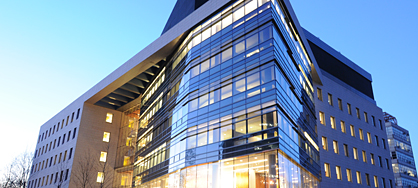
\includegraphics[width=4 cm]{fig/price.jpg}
    \end{column}
  \end{columns}
}

% outline 
%\AtBeginSection[]
%{
% \begin{frame}
%  \frametitle{Outline}
%  \small
%  \tableofcontents[currentsection,hideothersubsections]
%  \normalsize
% \end{frame}
%}
\AtBeginSection[]
{
  \begin{frame}
   \begin{multicols}{2}
   	 \small
     \tableofcontents[currentsection,hideothersubsections]
     \normalsize
   \end{multicols}
  \end{frame}
}

\begin{document}

	\begin{frame}
		\titlepage
	\end{frame}
	
	\begin{frame}
	\begin{block}{Status and Progress since last time}
	\begin{scriptsize}	
	\begin{itemize}
	\item Made friends with a category theorist and a couple more mathematicians
	\item Moved toward a clearer thesis question: What are the implications for evolution of combining current knowledge of stochasticity in gene expression and the topological structure of genotype-phenotype mappings? 
	\item Current answer: In accordance with the generalized `marginal problem'\footnote{\begin{tiny}
given a list of joint distributions of certain subsets of random variables $A_1, \ldots , A_n$, is it possible to find a joint distribution for all these variables, such that this distribution marginalizes to the given ones? One obvious necessary condition [sometimes referred to as the Kolmogorov consistency conditions] is that for any two of the given distributions which can be marginalized to the same subset of variables, the resulting marginals should be the same \cite{Fritz}
	\end{tiny}} , modularity in genotype-phenotype mappings can provide access to a relative superset of possible input-output (genotype-phenotype) relationships. Any environment consistently requiring genotype-phenotype relationships outside the space associated to the non-modular gene regulatory network architecture would induce infinite selective power in favor of various modular gene regulatory network architectures having access to these otherwise forbidden states.
	\item Data analysis: published 3 papers, worked on 2 more in collaboration with the Edelmann and Casadevall labs; 1 previous paper in collaboration with the Skoultchi lab
	\end{itemize}		
	\end{scriptsize}
	\end{block}
	\end{frame}

	\section[GP maps]{Genotype-phenotype mappings}
	% background on genotype-phenotype maps
% folder name: GPmaps

\begin{frame}
\begin{block}{}
An organism can be viewed as a collection of relatively fine-grained \textbf{genes} that are interpreted into phenotypes. If there are interaction constraints among the full set of genes the organism can be viewed as relatively coarse-grained \textbf{gene regulatory network modules}. 
\end{block}
\begin{block}{}
\textbf{Genotype-phenotype maps} can be evaluated at various levels of organization  beginning with a model of the gene and extending from simple molecular to ecosystem-level phenotypes.
\end{block}
\begin{block}{}
Repeated evaluation of the input-output dynamics of genotype-phenotype mappings on any given characteristic time-scale induces a \textbf{probability distribution over mappings} from \textbf{collections of genes} to \textbf{collections of phenotypes}. \textbf{Phenotypes} may be evaluated at any level, the level of evaluation determines the content of the collection of phenotype values.
\end{block}
\end{frame}
		
	\section[PDs of GPs]{Probability distributions of genotype-phenotype mappings}
    % spaces of genotype-phenotype maps
% probability distributions of genotype-phenotype maps
% folder name: PDsofGPs

% spaces of genotype-phenotype maps
\begin{frame}
The modeling description derives from \cite{Abramsky2011}.
\begin{block}{\textbf{Collection of subsets of a set}}
We denote the set of all subsets of a set $X$ as $\mathcal{P}(X)$.
\end{block}
\begin{block}{\textbf{Space of all genotype-phenotype maps}}
$\mathcal{P}(L)$ can then be viewed as a category in which the objects are subsets of genes and morphisms represent inclusion of a smaller subset into a larger superset (i.e. $U \subseteq U' \Rightarrow U \rightarrow U'$).
\end{block}
\begin{block}{\textbf{Inclusion vs Restriction}}
The category $\mathcal{P}(L)^{opp}$ then has the same objects, but the morphisms represent restriction from a larger to a smaller subset of genes (i.e. $U' \supseteq U \Rightarrow U' \rightarrow U$).
\end{block}
\end{frame}



\begin{frame}
In order to consider the set of all genotype-phenotype maps together, we can construct a functor $\mathcal{E}$
\begin{block}{\textbf{Space of all genotype-phenotype maps}}
The way in which the functor $\mathcal{E}$ acts on objects and morphisms $U$ and $U \subseteq U'$ respectively is
\begin{equation*}\label{eq:gpfunctor}
\begin{split}
\mathcal{E} \colon \mathcal{P}(L)^{opp} &\rightarrow Set,\\
U &\mapsto P^U,\\
U \subseteq U' &\mapsto res^{U'}_{U}.
\end{split}
\end{equation*}
\end{block}
So, the functor $\mathcal{E}$ takes a subset of genes and returns the set of genotype-phenotype mappings from the given subset of genes to the set of phenotypes.
\end{frame}

\begin{frame}
\begin{block}{\textbf{Space of all genotype-phenotype maps}}
The restriction map operates on sets deriving from the application of $\mathcal{E}$ to a subset of genes as follows
\begin{eqnarray*}
res^{U'}_{U} \colon \mathcal{E}(U') &\rightarrow& \mathcal{E}(U)\\
P^{U'} &\rightarrow& P^U\\
e' \colon U' \rightarrow P &\mapsto& e'|_U \colon U \rightarrow P
\end{eqnarray*}
$\mathcal{E}$ is thus, by definition, a presheaf functor, which is an object in the functor category $Sets^{\mathcal{P}(L)^{opp}}$.
\end{block}
\end{frame}

% distributions of genotype-phenotype maps
\begin{frame}
\begin{block}{\textbf{Space of distributions over genotype-phenotype maps}}
Given the presheaf functor, 
$$\mathcal{E} \colon \mathcal{P}(L)^{opp} \rightarrow Set,$$
mapping \textbf{genotypes} to the \textbf{set of maps} from those genotypes to the set of phenotypes, we can now compose it with the \textbf{distribution functor} $\mathcal{D}_R$ to obtain a new presheaf functor 
$$\mathcal{D}_R \circ \mathcal{E} \colon \mathcal{P}(L)^{opp} \rightarrow Set \rightarrow Set,$$
that assigns to each \textbf{genotype} a \textbf{distribution over the set of maps} from those genotypes to the set of possible phenotypes.
\end{block}
\end{frame}
\begin{frame}
\begin{block}{\textbf{Space of distributions over genotype-phenotype maps}}
The action of $\mathcal{D}_R \mathcal{E}$ on objects and morphisms in $\mathcal{P}(L)^{opp}$ yields
\begin{eqnarray*}
\mathcal{D}_R \mathcal{E} \colon \mathcal{P}(L)^{opp} &\rightarrow& Set,\\
U &\mapsto& \mathcal{D}_R \mathcal{E}(U) \equiv d \colon P^U \rightarrow R,\\
U \subseteq U' &\mapsto& \mathcal{D}_R \mathcal{E}(U') \rightarrow \mathcal{D}_R \mathcal{E}(U).
\end{eqnarray*}
\end{block}
\end{frame}


\begin{frame}
\begin{block}{\textbf{Space of distributions over genotype-phenotype maps}}
where
\begin{eqnarray*}
\mathcal{D}_R \mathcal{E}(U') &\rightarrow& \mathcal{D}_R \mathcal{E}(U),\\
d \colon P^{U'} \rightarrow R &\rightarrow& d|U \colon P^{U} \rightarrow R
\end{eqnarray*}
and
\begin{eqnarray*}
d \colon P^{U'} &\rightarrow& R,\\
s' &\mapsto& d(s');\\
d|U \colon P^{U} &\rightarrow& R,\\
s &\mapsto& \sum_{s' \in \mathcal{E}(U'),\, s'|U=s} d(s').
\end{eqnarray*}
\end{block}
\end{frame}


% definition of the underlying distribution functor
%\begin{frame}
For the case in which we consider $R$ to be the semiring of non-negative real numbers $\left( \mathbb{R}_{\geq 0},+,0,\times,1 \right)$, $\mathcal{D}_R (L)$ represents the set of probability distributions on the set $L$.

We can consider the set of all (probability) distributions defined on the set $L$ as being given by a functor applied to $L$ as $\mathcal{D}_R (L)$. We can again explicitly represent the way in which the functor $\mathcal{D}_R$ acts on objects and morphisms $L$ and $f \colon L \rightarrow M$ as
\end{frame}

\begin{frame}
\begin{block}{\textbf{Distribution functor}}
where
\begin{equation}\label{eq:distfunctor}
\begin{split}
\mathcal{D}_R \colon Set &\rightarrow Set,\\
L &\mapsto \mathcal{D}_R (L),\\
f \colon L \rightarrow M &\mapsto \mathcal{D}_R (f) \colon \mathcal{D}_R (L) \rightarrow \mathcal{D}_R (M),
\end{split}
\end{equation}
and
\begin{eqnarray*}
\mathcal{D}_R (f) \colon \mathcal{D}_R (L) &\rightarrow& \mathcal{D}_R (M),\\
d &\mapsto& \left[ m \mapsto \sum_{f(l)=m} d(l) \right].
\end{eqnarray*}
\end{block}
\end{frame}

% example of global distribution
\begin{frame}
\begin{columns}[c]
\begin{column}{0.5\textwidth}
\begin{block}{\textbf{Example: 4 gene model}}
\begin{eqnarray*}
L \in \mathcal{P}(L) &=& \{l_1,l_2,l'_1,l'_2\}\\
P &=& \{0,1\}\\
\mathcal{E}(L) &=& P^L\\
R &=& \mathbb{R}_{\geq 0}\\
\mathcal{D}_R \mathcal{E}(L) &=& \{d | d \colon P^L \rightarrow R \}\\
\sum_{e \in P^L} d(e) &=& 1
\end{eqnarray*}
\end{block}
\end{column}
\begin{column}{0.5\textwidth}
\begin{table}
\centering
\begin{tabular}{ r || c }
$l_1 l_2 l'_1 l'_2$ & probability \\ \hline
0000 & $q_1$ \\
0010 & $q_2$ \\
0001 & $q_3$ \\
0011 & $q_4$ \\
1000 & $q_5$ \\
1010 & $q_6$ \\
1001 & $q_7$ \\
1011 & $q_8$ \\
0100 & $q_9$ \\
0110 & $q_{10}$ \\
0101 & $q_{11}$ \\
0111 & $q_{12}$ \\
1100 & $q_{13}$ \\
1110 & $q_{14}$ \\
1101 & $q_{15}$ \\
1111 & $q_{16}$
\end{tabular}
%\caption{Example of a distribution defined on the collection of maps from the set of all possible alleles, $L$, to the set of phenotype values, $P$. Such a distribution may be an instance of a global section $d \in \mathcal{D}_R\mathcal{E}(L)$ if it satisfies the sheaf condition.  Here each row represents the probability assigned to a map in the collection of maps given by the set $P^L$. For example, $P[l_1=0,l_2=0,l'_1=0,l'_2=0]=q_1$ gives the probability associated to the map $\{l_1, l_2, l'_1, l'_2\} \mapsto \{0,0,0,0\}$.}
%\label{tab:hidvarmod}
\end{table}
\end{column}
\end{columns}
\end{frame}



	\section[Modular GPs]{Modular genotype-phenotype maps}
	% modularization of genotype-phenotype maps
% probability distributions of genotype-phenotype maps
% folder name: ModularGPs

% spaces of genotype-phenotype maps
\begin{frame}
How is the model modified by information indicating that the genotype space is fundamentally decomposed into modules\footnote{also referred to as overlapping subsets'}?
\begin{center}
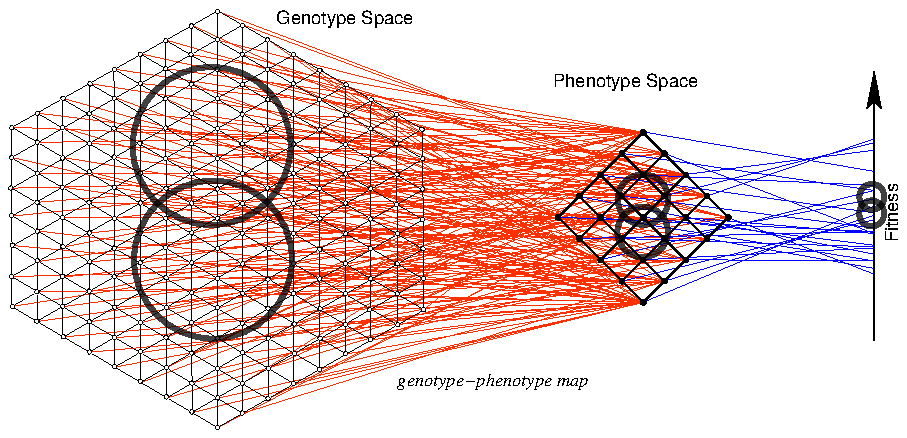
\includegraphics[width=0.8\textwidth]{fig/gpmapmod.pdf}\\
$e \colon U \longrightarrow P$, $e' \colon U' \longrightarrow P$, $U \cap U' \neq \emptyset$
\end{center}
% \begin{eqnarray*}
% e \colon U \longrightarrow P\\
% e' \colon U' \longrightarrow P\\
% U \cap U' \neq \emptyset
% \end{eqnarray*}
\end{frame}


	
	\section[GMs]{Graphical models}
	% graphical models
% relationships between graphical models and probability
% relationships between graphical models and polytopes
% folder name: GraphicalModels

% graphicalmodels
\begin{frame}
\begin{block}{\textbf{Question}}
How can we summarize models like this in a manner that enables us to \textbf{derive the associated constraints} automatically from the model description so that we can \textbf{compare alternative models}?
\end{block}
\begin{block}{\textbf{Example: 4 gene model (C4 constraints)}}
\begin{equation*}
\begin{aligned}
& L \in \mathcal{P}(L) = \{l_1,l_2,l'_1,l'_2\}\\
& \mathcal{G} = \{\{l_1,l_2 \},\{l_1,l'_2 \},\{l'_1,l_2\},\{l'_1,l'_2\} \}\\
& P = \{0,1\}\\
& \coprod_{O \in \mathcal{G}} \mathcal{E}(O) = \{e \colon O \rightarrow P | O \in \mathcal{G} \}\\
& R = \mathbb{R}_{\geq 0}\\
& \coprod_{O \in \mathcal{G}} \mathcal{D}_R\mathcal{E}(O) = \{d_O \colon P^O \rightarrow R | O \in \mathcal{G} \}\\
& \forall O \in \mathcal{G} \left[ \sum_{e \in P^O} d_O(e) = 1 \right]
\end{aligned}
\end{equation*}
\end{block}
\end{frame}

\begin{frame}
\begin{block}{\textbf{Question}}
How can we summarize models like this in a manner that enables us to \textbf{derive the associated constraints} automatically from the model description so that we can \textbf{compare alternative models}?
\end{block}
\begin{block}{\textbf{Graphical models}}
For example, for the cover of genotype space given by
$\mathcal{G} = \{\{l_1,l_2 \},\{l_1,l'_2 \},\{l'_1,l_2\},\{l'_1,l'_2\} \}$
there is an associated graph, in this case the 4-cycle (also referred to as C4):
\begin{center}
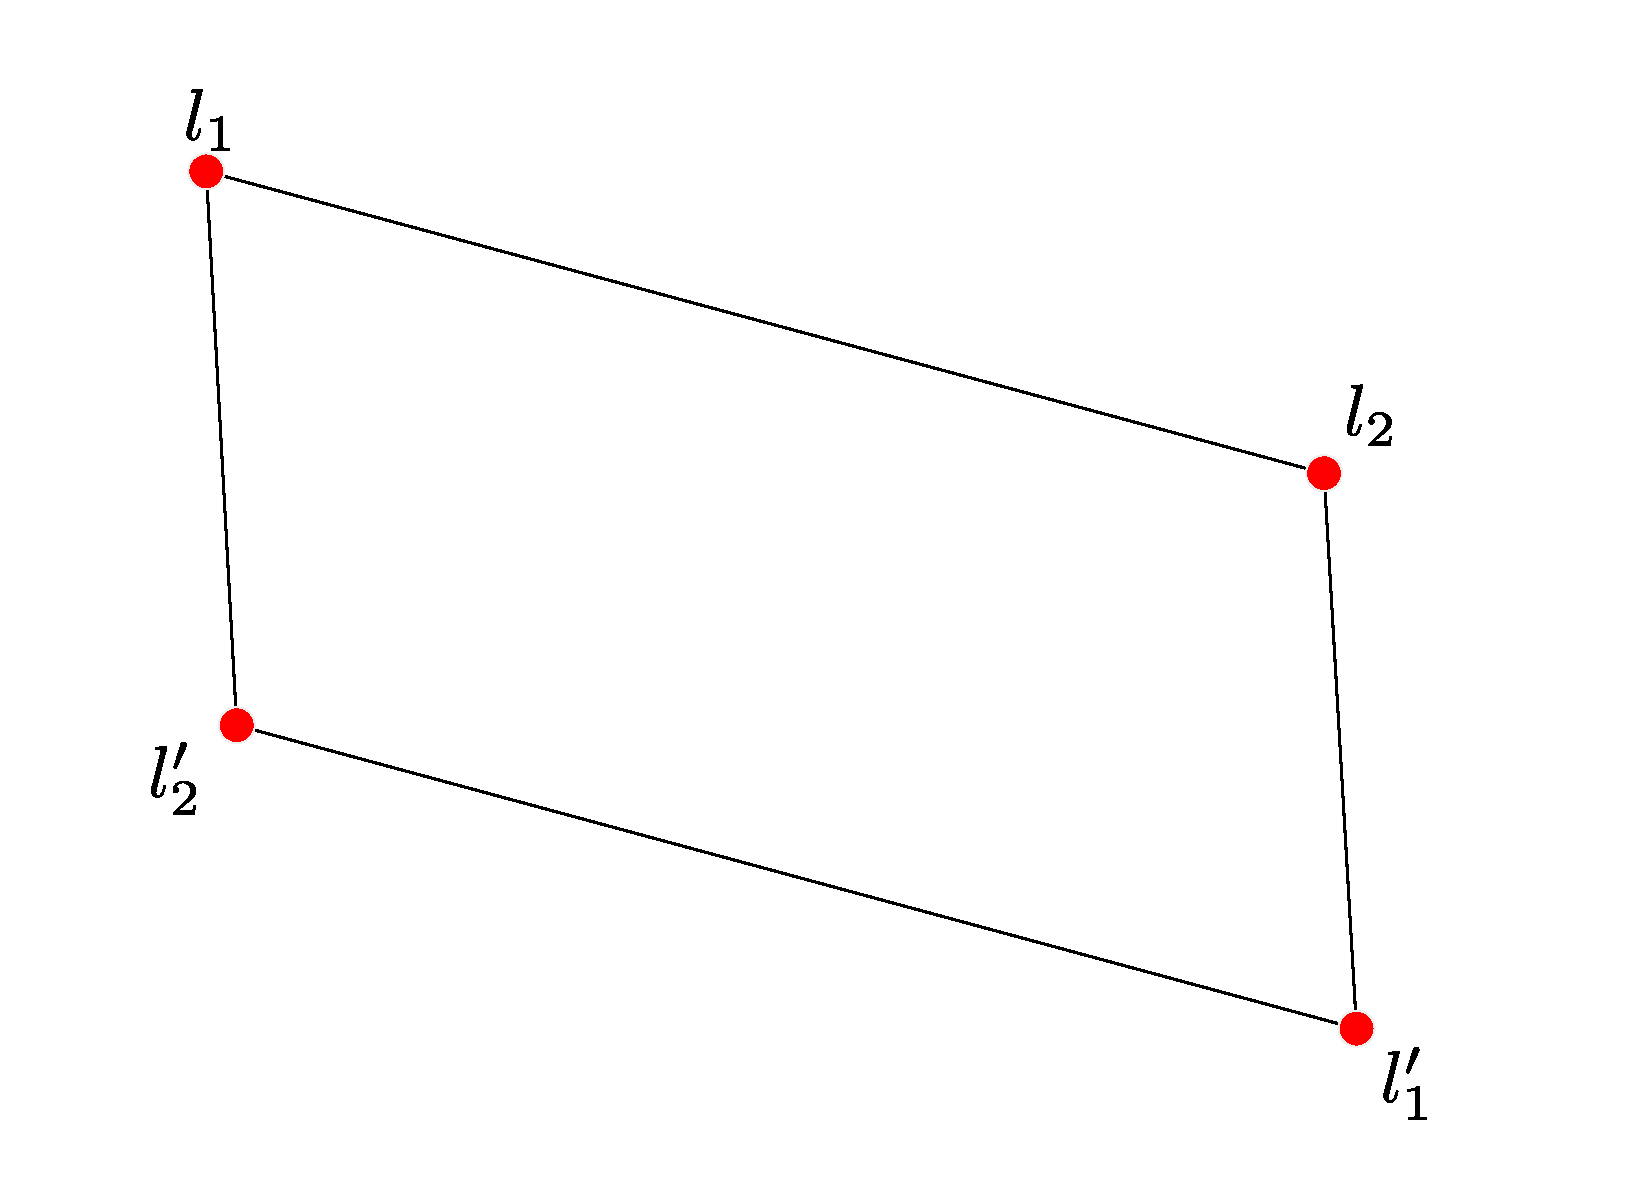
\includegraphics[width=0.4\textwidth]{fig/C4graph_labelled.pdf}
\end{center}
\end{block}
\end{frame}


\begin{frame}
For a cover of the genotype space, $\mathcal{G}$ associated to a graph, we can construct an incidence matrix, $\mathbf{G}$, representing the relationship between genotype-phenotype mappings having as domain particular GRNM contexts given by the $O \in \mathcal{G}$ and those global genotype-phenotype mappings defined on $L$.

\begin{block}{\textbf{Marginalization matrix associated to a graph}}
This is equivalent to the statement that there is some binary relation,
\begin{equation*}
R \subseteq \mathcal{E}(L) \times \coprod_{O \in \mathcal{G}} \mathcal{E}(O),
\end{equation*}
whose logical matrix representation, $\mathbf{G}$, we would like to construct.
\end{block}
\end{frame}

\begin{frame}
In the first case, $\mathcal{E}(L) = P^L$ we have $\{t_1, \ldots t_m\} = \{t_j | t_j \in P^L\}$. In the second case, $\coprod_{O \in \mathcal{G}} \mathcal{E}(O)$, we have $\{e_1, \ldots e_n\} = \coprod_{O \in \mathcal{G}} \mathcal{E}(O)$. So we have two sets of maps, one defined on $P^L$ and the other defined on $\mathcal{E}(O) = P^O$ for each $O \in \mathcal{G}$. This yields a method of specifying the intended relationship that defines $\mathbf{G}_{n \times m}$ in terms of $t_j \in P^L$ and $e_i \in \mathcal{E}(O)$ :
\begin{eqnarray*}
\mathbf{G}[i,j] =
\begin{cases}
1, & t_j|O = e_i,\\
0, & \text{otherwise}.
\end{cases}
\end{eqnarray*}
\end{frame}

\begin{frame}
This matrix can be viewed as an operator acting via matrix multiplication on distributions
\begin{eqnarray*}
\mathbf{G} \colon \mathcal{D}_R\mathcal{E}(L) &\rightarrow& \mathcal{D}_R\mathcal{E}(\mathcal{G}),\\
d &\mapsto& (d|O)_{O \in \mathcal{G}},
\end{eqnarray*}
and thereby taking a global distribution defined on genotype-phenotype maps whose domain is the full set of genes $L$ to the \emph{marginalized} distributions that are defined relative to gene regulatory network modules contained in a covering of the genotype space $\mathcal{G}$.
\end{frame}


\begin{frame}
In terms of the probability values the resulting system of equations $\mathbf{G}_{n \times m} \mathbf{Q}_{m \times 1} = \mathbf{P}_{n \times 1}$ is
\begin{equation*}
\begin{aligned}\label{eq:globsys}
p_1 &= q_1 + q_2 + q_3 + q_4 &
p_2 &= q_5 + q_6 + q_7 + q_8 \\
p_3 &= q_9 + q_{10} + q_{11} + q_{12} &
p_4 &= q_{13} + q_{14} + q_{15} + q_{16}\\
p_5 &= q_1 + q_3 + q_5 + q_7 &
p_6 &= q_2 + q_4 + q_6 + q_8 \\
p_7 &= q_9 + q_{11} + q_{13} + q_{15} &
p_8 &= q_{10} + q_{12} + q_{14} + q_{16}\\
p_9 &= q_1 + q_2 + q_9 + q_{10} &
p_{10} &= q_5 + q_6 + q_{13} + q_{14} \\
p_{11} &= q_3 + q_4 + q_{11} + q_{12} &
p_{12} &= q_7 + q_8 + q_{15} + q_{16}\\
p_{13} &= q_1 + q_5 + q_{9} + q_{13} &
p_{14} &= q_2 + q_6 + q_{10} + q_{14} \\
p_{15} &= q_3 + q_7 + q_{11} + q_{15} &
p_{16} &= q_4 + q_8 + q_{12} + q_{16}
\end{aligned}
\end{equation*}
\end{frame}

\begin{frame}
For the previously defined model with $\mathcal{G} = \{\{l_1,l_2 \},\{l_1,l'_2 \},\{l'_1,l_2\},\{l'_1,l'_2\} \}$, $\mathbf{G}$ is
\begin{center}
%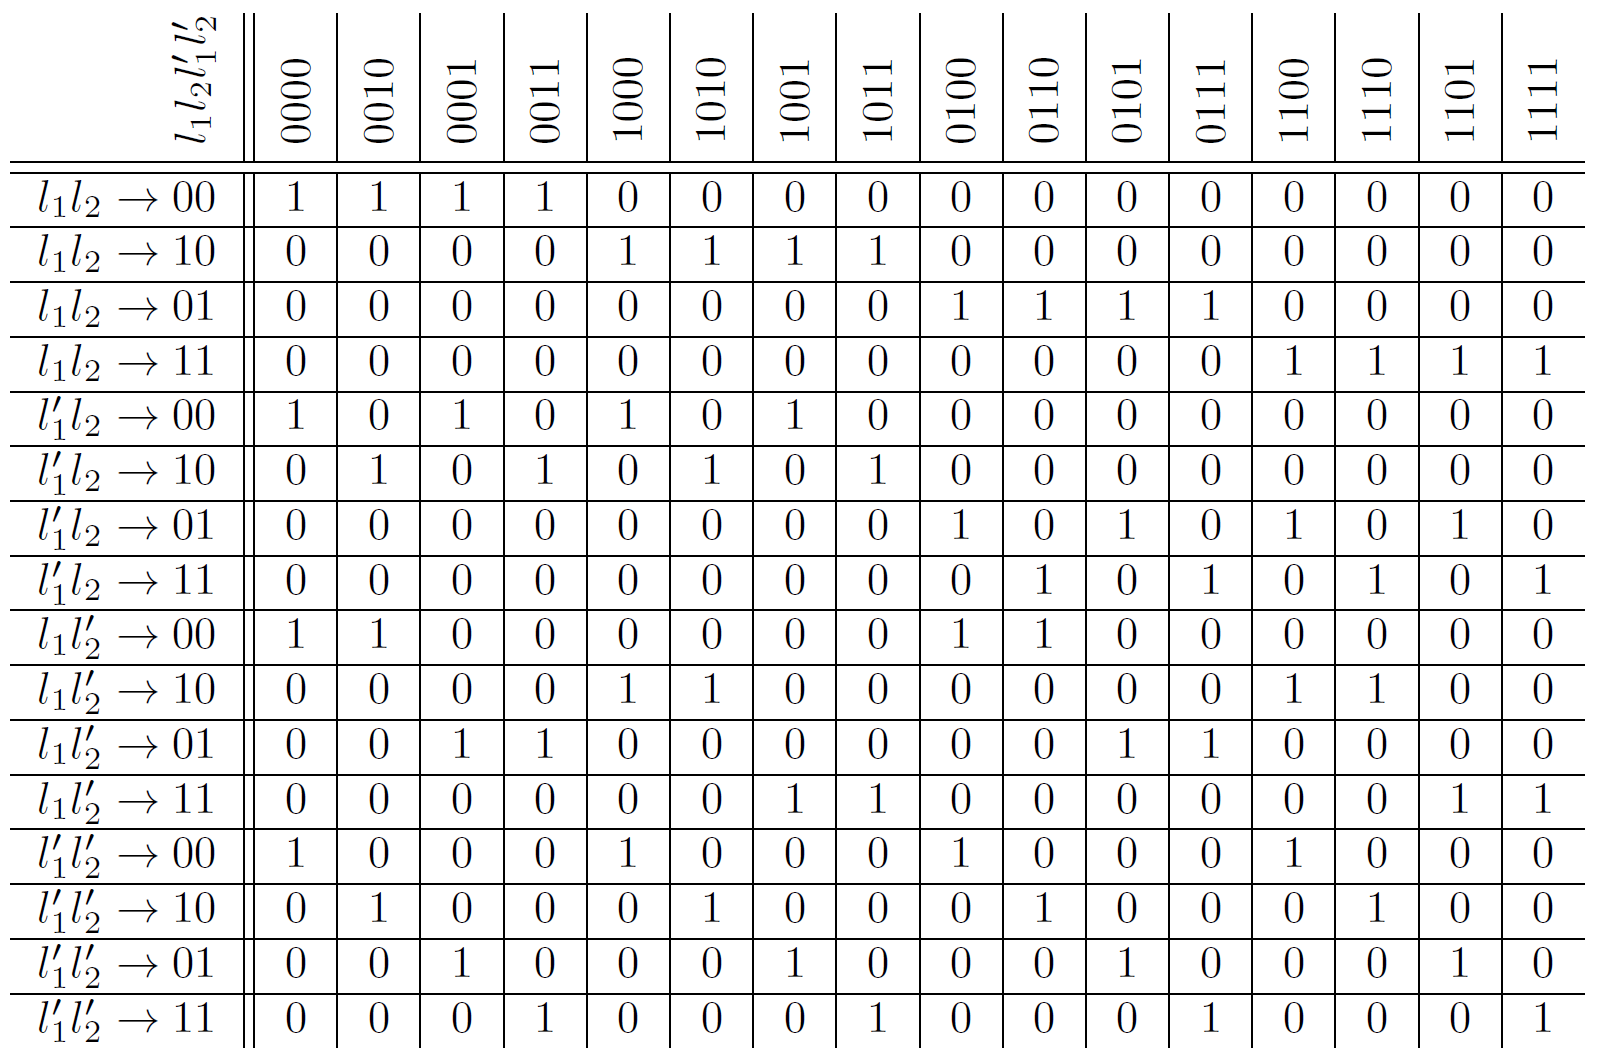
\includegraphics[width=0.9\textwidth]{fig/Gmat.png}
\begin{tiny}
%!TEX root = ../plos_template.tex
\begin{table}[!ht]
\centering
\begin{tabular}{ r || c | c | c | c | c | c | c | c | c | c | c | c | c | c | c | c }
		 &	\begin{sideways}$e^{1234}_{0000}$\end{sideways} & \begin{sideways}$e^{1234}_{0010}$\end{sideways} & \begin{sideways}$e^{1234}_{0001}$\end{sideways} & \begin{sideways}$e^{1234}_{0011}$\end{sideways}
			  & \begin{sideways}$e^{1234}_{1000}$\end{sideways} & \begin{sideways}$e^{1234}_{1010}$\end{sideways} & \begin{sideways}$e^{1234}_{1001}$\end{sideways} & \begin{sideways}$e^{1234}_{1011}$\end{sideways}
			  &	\begin{sideways}$e^{1234}_{0100}$\end{sideways} & \begin{sideways}$e^{1234}_{0110}$\end{sideways} & \begin{sideways}$e^{1234}_{0101}$\end{sideways} & \begin{sideways}$e^{1234}_{0111}$\end{sideways}
			  &	\begin{sideways}$e^{1234}_{1100}$\end{sideways} & \begin{sideways}$e^{1234}_{1110}$\end{sideways} & \begin{sideways}$e^{1234}_{1101}$\end{sideways} & \begin{sideways}$e^{1234}_{1111}$\end{sideways}\\ \hline \hline
    $e^{12}_{00}$ & 1 & 1 & 1 & 1 & 0 & 0 & 0 & 0 & 0 & 0 & 0 & 0 & 0 & 0 & 0 & 0\\ \hline
    $e^{12}_{10}$ & 0 & 0 & 0 & 0 & 1 & 1 & 1 & 1 & 0 & 0 & 0 & 0 & 0 & 0 & 0 & 0\\ \hline
    $e^{12}_{01}$ & 0 & 0 & 0 & 0 & 0 & 0 & 0 & 0 & 1 & 1 & 1 & 1 &  0 & 0 & 0 & 0\\ \hline
    $e^{12}_{11}$ & 0 & 0 & 0 & 0 & 0 & 0 & 0 & 0 & 0 & 0 & 0 & 0 & 1 & 1 & 1 & 1\\ \hline

    $e^{32}_{00}$ & 1 & 0 & 1 & 0 & 1 & 0 & 1 & 0 & 0 & 0 & 0 & 0 & 0 & 0 & 0 & 0\\ \hline
    $e^{32}_{10}$ & 0 & 1 & 0 & 1 & 0 & 1 & 0 & 1 & 0 & 0 & 0 & 0 & 0 & 0 & 0 & 0\\ \hline
    $e^{32}_{01}$ & 0 & 0 & 0 & 0 & 0 & 0 & 0 & 0 & 1 & 0 & 1 & 0 & 1 & 0 & 1 & 0\\ \hline
    $e^{32}_{11}$ & 0 & 0 & 0 & 0 & 0 & 0 & 0 & 0 & 0 & 1 & 0 & 1 & 0 & 1 & 0 & 1\\ \hline

    $e^{14}_{00}$ & 1 & 1 & 0 & 0 & 0 & 0 & 0 & 0 & 1 & 1 & 0 & 0 & 0 & 0 & 0 & 0\\ \hline
    $e^{14}_{10}$ & 0 & 0 & 0 & 0 & 1 & 1 & 0 & 0 & 0 & 0 & 0 & 0 & 1 & 1 & 0 & 0\\ \hline
    $e^{14}_{01}$ & 0 & 0 & 1 & 1 & 0 & 0 & 0 & 0 & 0 & 0 & 1 & 1 & 0 & 0 & 0 & 0\\ \hline
    $e^{14}_{11}$ & 0 & 0 & 0 & 0 & 0 & 0 & 1 & 1 & 0 & 0 & 0 & 0 & 0 & 0 & 1 & 1\\ \hline

    $e^{34}_{00}$ & 1 & 0 & 0 & 0 & 1 & 0 & 0 & 0 & 1 & 0 & 0 & 0 & 1 & 0 & 0 & 0\\ \hline
    $e^{34}_{10}$ & 0 & 1 & 0 & 0 & 0 & 1 & 0 & 0 & 0 & 1 & 0 & 0 & 0 & 1 & 0 & 0\\ \hline
    $e^{34}_{01}$ & 0 & 0 & 1 & 0 & 0 & 0 & 1 & 0 & 0 & 0 & 1 & 0 & 0 & 0 & 1 & 0\\ \hline
    $e^{34}_{11}$ & 0 & 0 & 0 & 1 & 0 & 0 & 0 & 1 & 0 & 0 & 0 & 1 & 0 & 0 & 0 & 1\\
    \end{tabular}
\caption{Explicit construction of $\mathbf{G}_{n \times m}$ for the case $L = \{ l_1,l_2,l_3,l_4 \}$, $\mathcal{G} = \{\{l_1,l_2 \},\{l_1,l_4 \},\{l_3,l_2\},\{l_3,l_4\} \}$, $P=\{0,1\}$ and thus $\mathbf{G}_{(2 \cdot 2)^2 \times 2^{2 \cdot 2}} = \mathbf{G}_{16 \times 16}$.}
\label{tab:logmat222}
\end{table}

\end{tiny}
\end{center}
\end{frame}


\begin{frame}
\begin{block}{\textbf{Question}}
How can we find the constraints on $\mathbf{P}_{n \times 1}$ in order for $\mathbf{G}_{n \times m} \mathbf{Q}_{m \times 1} = \mathbf{P}_{n \times 1}$ to have a solution?
\end{block}
\begin{block}{\textbf{Cokernel}}
These constraints are defined by the cokernel of $\mathbf{G} \colon \mathcal{D}_R\mathcal{E}(L) \rightarrow \mathcal{D}_R\mathcal{E}(\mathcal{G})$
\begin{center}
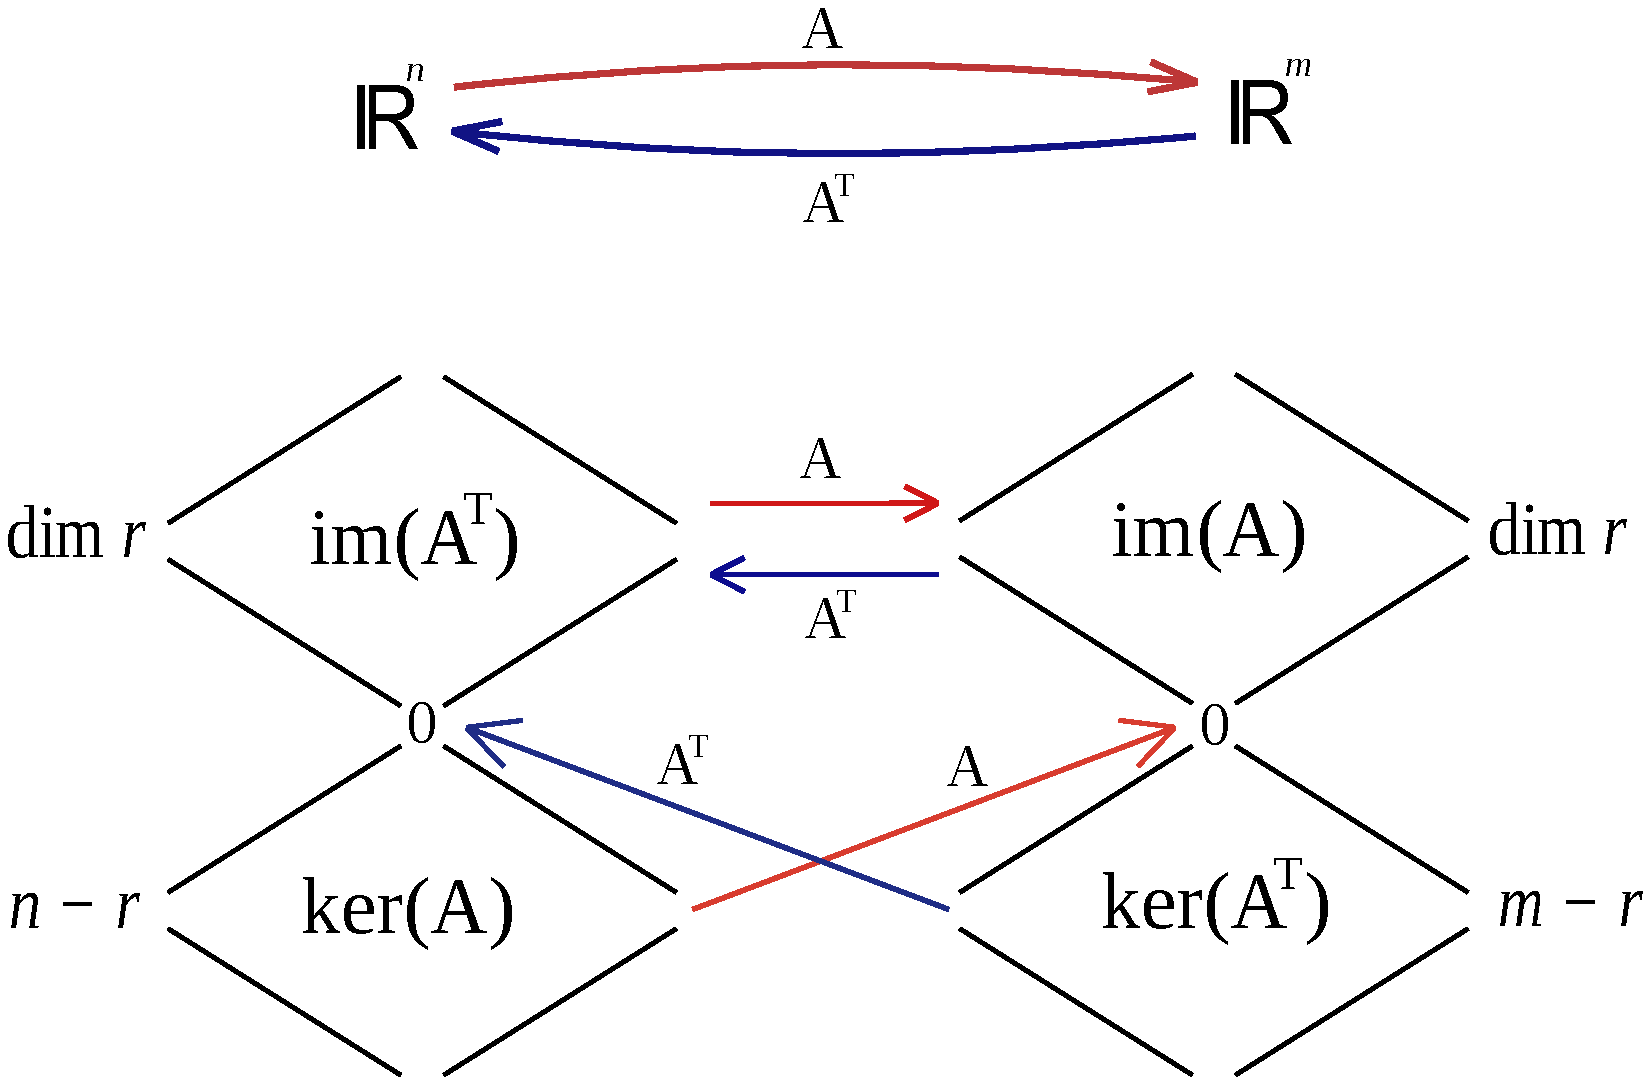
\includegraphics[width=0.5\textwidth]{fig/fundamental_subspaces.pdf}
\end{center}
\end{block}
\end{frame}






	\section[PTs and PDs]{Polytopes and (sub)spaces of probability distributions}
	% background on polytopes
% folder name: PTsandPDs

\begin{frame}
\begin{block}{\textbf{Question}}
How can we find the constraints on $\mathbf{P}_{n \times 1}$ in order for $\mathbf{G}_{n \times m} \mathbf{Q}_{m \times 1} = \mathbf{P}_{n \times 1}$ to have a solution?
\end{block}
\begin{block}{\textbf{Cokernel}}
These constraints are defined by the cokernel of $\mathbf{G} \colon \mathcal{D}_R\mathcal{E}(L) \rightarrow \mathcal{D}_R\mathcal{E}(\mathcal{G})$
\begin{center}
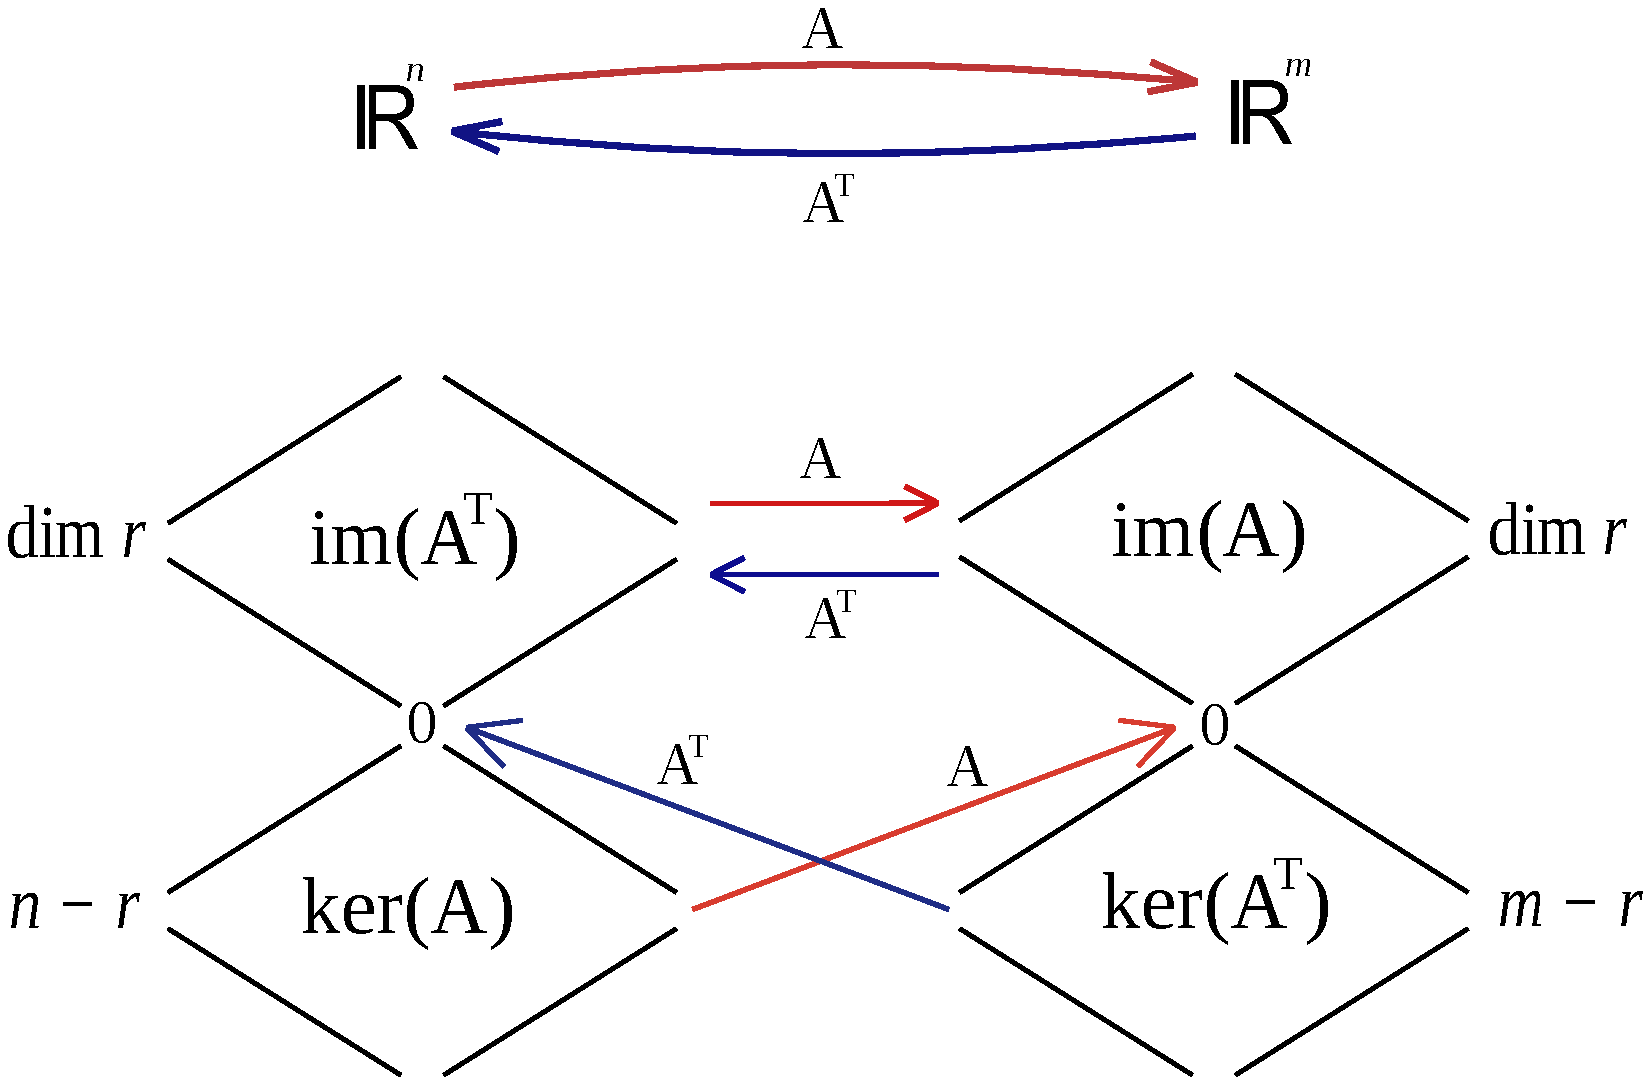
\includegraphics[width=0.5\textwidth]{fig/fundamental_subspaces.pdf}
\end{center}
\end{block}
\end{frame}


\begin{frame}
\begin{block}{\textbf{Question}}
How can we interpret these relationships geometrically?
\end{block}
\begin{block}{\textbf{Polytopes of probability distributions}}
Spaces of probability distributions and constraints placed upon them by linear transformations like G give rise to polytopes
\end{block}
\begin{block}{\textbf{Polytope}}
\begin{center}
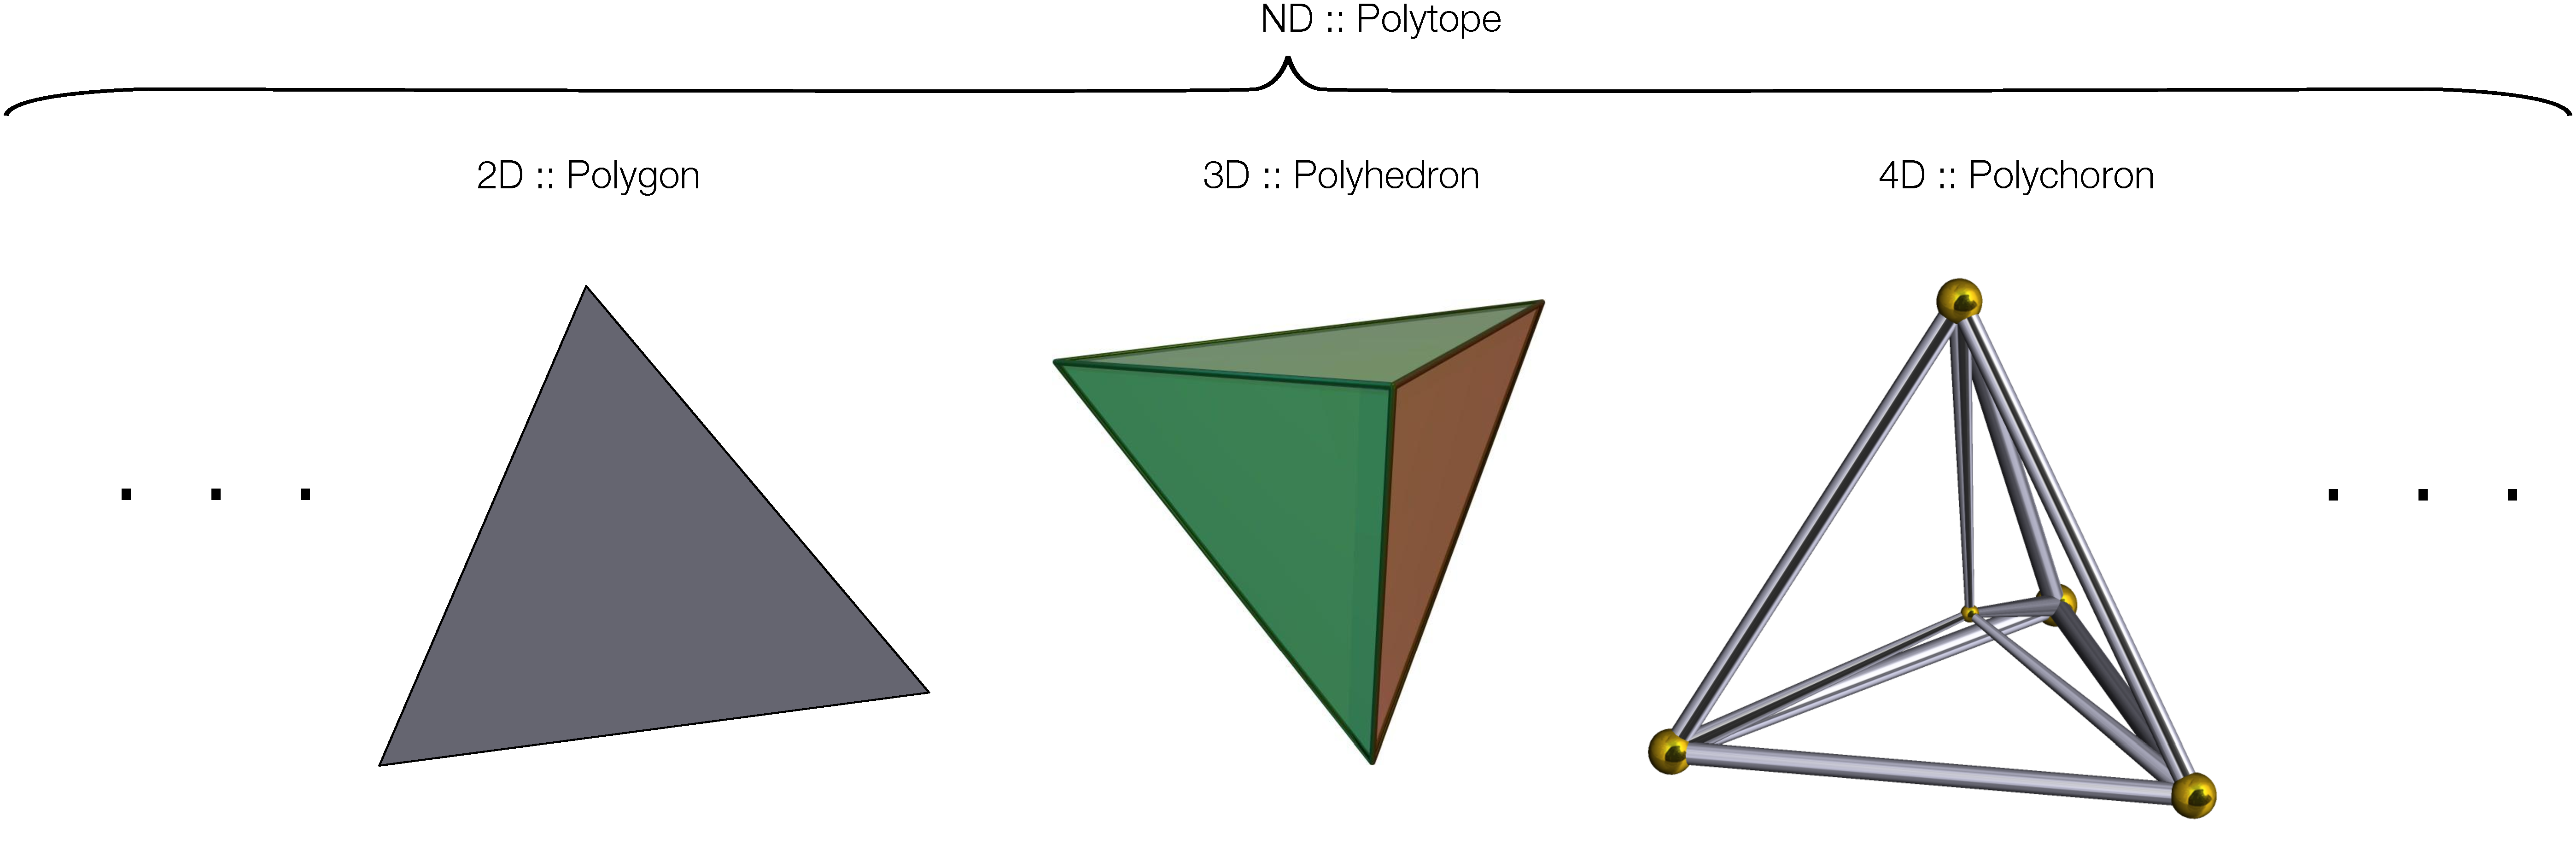
\includegraphics[width=0.9\textwidth]{fig/polytope.pdf}
\end{center}
\end{block}
\end{frame}


\begin{frame}
\begin{block}{\textbf{Constrained spaces of probability distributions}}
\begin{center}
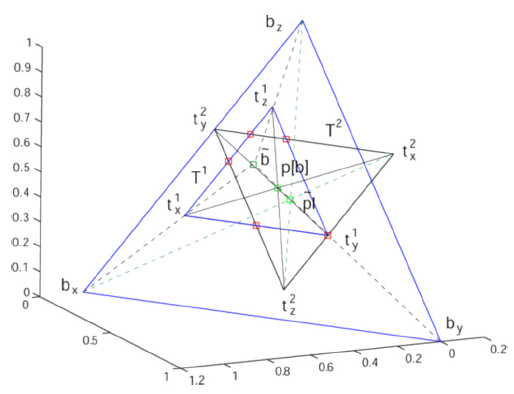
\includegraphics[width=0.5\textwidth]{fig/intersectingprobdists.png}
\end{center}
\end{block}
\end{frame}
\begin{frame}
Spaces of probability distributions and constraints placed upon them by linear transformations like G give rise to polytopes
\begin{block}{\textbf{Polytope}}
\textbf{Convex polytopes} can be represented in two different but equivalent forms. The so-called \textbf{H-representation} in terms of the set of solutions of a system of linear inequalities
$$K\mathbf{x} \geq \mathbf{b}$$
or the so-called \textbf{V-representation} in terms of the convex hull
$$\left\{ \mathbf{x} \in \mathbb{R}^d | \mathbf{x} = \sum_{i=1}^n \lambda_i \mathbf{x_i}, \lambda_i \in \mathbb{R}, \lambda_i \geq 0, \sum_{i=1}^n \lambda_i = 1  \right\} $$
of a finite set of points.
\end{block}
\end{frame}

\begin{frame}
\begin{columns}[t]
\begin{column}{0.5\textwidth}
\begin{block}{\textbf{2-simplex}}
H-representation
\begin{equation*}
\begin{aligned}\label{eq:simplex2H}
1 &\geq x_1 + x_2\\ 
x_1 &\geq 0\\
x_2 &\geq 0
\end{aligned}
\end{equation*}
V-representation
$$
\begin{bmatrix}
  1 & 0 & 0\\
  1 & 1 & 0\\
  1 & 0 & 1\\
\end{bmatrix}
$$
\end{block}
\end{column}
\begin{column}{0.5\textwidth}
\begin{center}
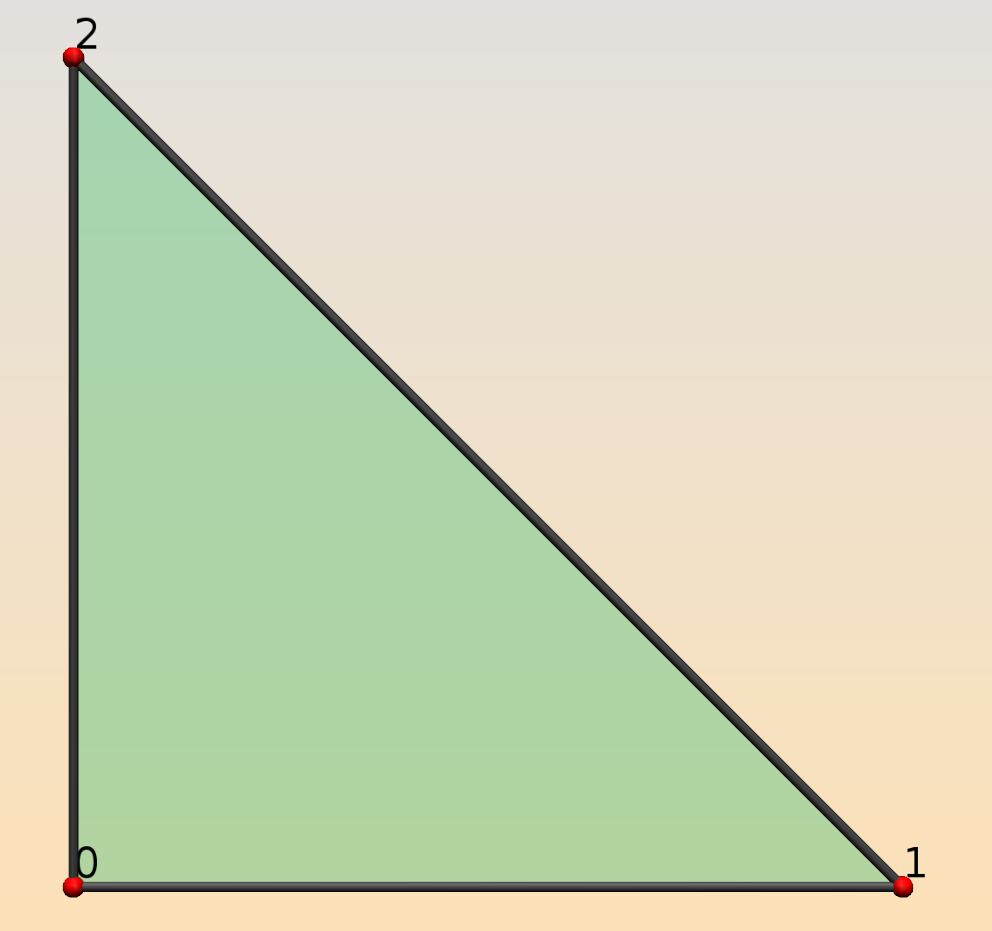
\includegraphics[width=1.0\textwidth]{fig/simplex2.png}
\end{center}
\end{column}
\end{columns}
\end{frame}

\begin{frame}
\begin{columns}[t]
\begin{column}{0.5\textwidth}
\begin{block}{\textbf{3-simplex}}
H-representation
\begin{equation*}
\begin{aligned}\label{eq:simplex3H}
1 &\geq x_1 + x_2 + x_3\\
x_1 &\geq 0\\
x_2 &\geq 0\\
x_3 &\geq 0
\end{aligned}
\end{equation*}
V-representation
$$
\begin{bmatrix}
  1 & 0 & 0 & 0\\
  1 & 1 & 0 & 0\\
  1 & 0 & 1 & 0\\
  1 & 0 & 0 & 1\\
\end{bmatrix}
$$
\end{block}
\end{column}
\begin{column}{0.5\textwidth}
\begin{center}
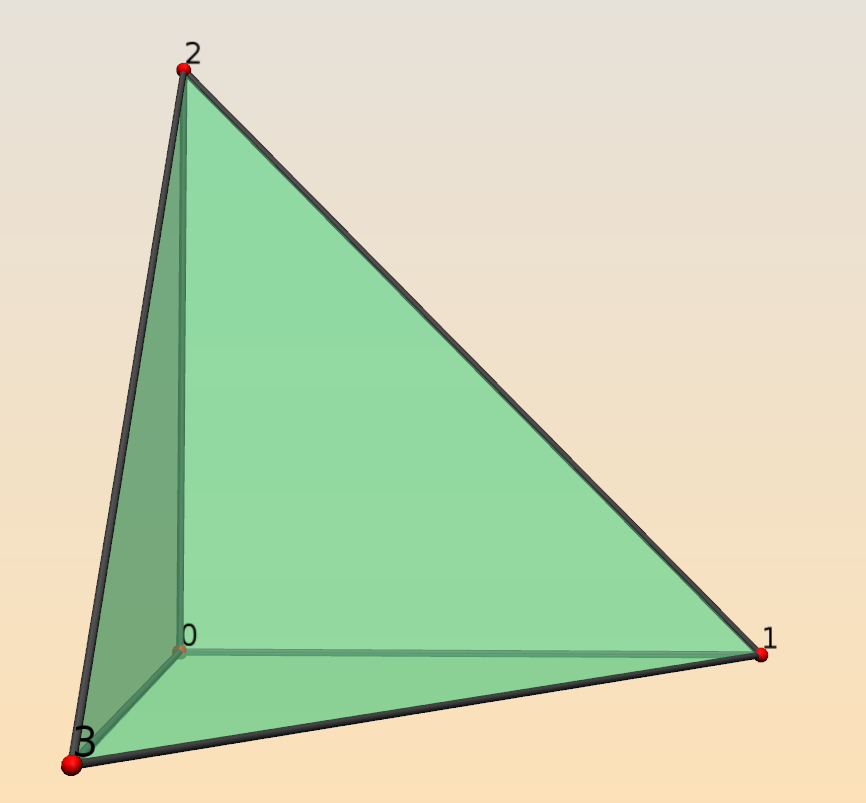
\includegraphics[width=1.0\textwidth]{fig/simplex3.png}
\end{center}
\end{column}
\end{columns}
\end{frame}

%!TEX root = ../../beamer.tex
\begin{frame}
\begin{block}{\textbf{Probability simplex}}
$$
\Delta_{m-1} = \left\{ (p_1, \ldots , p_m) \in \mathbb{R}^m \colon \sum_{i=1}^m p_i = 1 \text{ and } p_j \geq 0 \text{ for all } j \right\}.
$$
\end{block}
\begin{block}{\textbf{Relating spaces of probability distributions}}
In examples we can be more explicit about the geometry of the domain and codomain of the linear transformation
$$\mathbf{G} \colon \mathcal{D}_R\mathcal{E}(L) \rightarrow \mathcal{D}_R\mathcal{E}(\mathcal{G}).$$
In the example $(2,2,2)$ or C4 case we are interested in linear transformations
$$
G \colon \Delta_{15} \longrightarrow \Delta_3^{\oplus 4},
$$
where $(q_1, \ldots, q_{16}) \in \Delta_{15}$ and $((p_1, \ldots , p_4), \ldots, (p_{13},\ldots,p_{16})) \in \Delta_3 \oplus \Delta_3 \oplus \Delta_3 \oplus \Delta_3$.
\end{block}
\end{frame}


\begin{frame}
\begin{block}{\textbf{Question}}
How can we find the constraints on $\mathbf{P}_{n \times 1}$ in order for $\mathbf{G}_{n \times m} \mathbf{Q}_{m \times 1} = \mathbf{P}_{n \times 1}$ to have a solution?
\end{block}
\begin{block}{\textbf{Cokernel of $\mathbf{G}$ + normalization constraints}}
\begin{tiny}
\begin{equation*}\label{eq:eqmat}
\begin{aligned}
\begin{bmatrix}
  -1 & -1 & 0 & 0 & 1 & 1 & 0 & 0 & 0 & 0 & 0 & 0 & 0 & 0 & 0 & 0 & 0\\
  0 & 0 & -1 & -1 & 0 & 0 & 1 & 1 & 0 & 0 & 0 & 0 & 0 & 0 & 0 & 0 & 0\\
  -1 & 0 & -1 & 0 & 0 & 0 & 0 & 0 & 1 & 1 & 0 & 0 & 0 & 0 & 0 & 0 & 0\\
  0 & -1 & 0 & -1 & 0 & 0 & 0 & 0 & 0 & 0 & 1 & 1 & 0 & 0 & 0 & 0 & 0\\
  0 & 0 & 0 & 0 & 0 & 0 & 0 & 0 & -1 & 0 & -1 & 0 & 1 & 1 & 0 & 0 & 0\\
  0 & 0 & 0 & 0 & -1 & 0 & -1 & 0 & 0 & 0 & 0 & 0 & 1 & 0 & 1 & 0 & 0\\
  -1 & -1 & -1 & -1 & 1 & 0 & 1 & 0 & 1 & 0 & 1 & 0 & -1 & 0 & 0 & 1 & 0\\
  1 & 1 & 1 & 1 & 0 & 0 & 0 & 0 & 0 & 0 & 0 & 0 & 0 & 0 & 0 & 0 & 1\\
  0 & 0 & 0 & 0 & 1 & 1 & 1 & 1 & 0 & 0 & 0 & 0 & 0 & 0 & 0 & 0 & 1\\
  0 & 0 & 0 & 0 & 0 & 0 & 0 & 0 & 1 & 1 & 1 & 1 & 0 & 0 & 0 & 0 & 1\\
  0 & 0 & 0 & 0 & 0 & 0 & 0 & 0 & 0 & 0 & 0 & 0 & 1 & 1 & 1 & 1 & 1\\
\end{bmatrix}
\end{aligned}
\end{equation*}
\end{tiny}
\end{block}
\end{frame}

\begin{frame}
\begin{block}{\textbf{reduced Cokernel of $\mathbf{G}$ + normalization constraints}}
\begin{tiny}
\begin{equation*}\label{eq:eqmat}
\begin{aligned}
\begin{bmatrix}
   1 & 0 & 0 & -1 & 0 & 0 & 1 & 1 & 0 & 0 & 1 & 1 & 0 & 0 & 0 & 0 & 1\\
  0 & 1 & 0 & 1 & 0 & 0 & 0 & 0 & 0 & 0 & -1 & -1 & 0 & 0 & 0 & 0 & 0\\
  0 & 0 & 1 & 1 & 0 & 0 & -1 & -1 & 0 & 0 & 0 & 0 & 0 & 0 & 0 & 0 & 0\\
  0 & 0 & 0 & 0 & 1 & 0 & 1 & 0 & 0 & 0 & 0 & 0 & 0 & 1 & 0 & 1 & 1\\
  0 & 0 & 0 & 0 & 0 & 1 & 0 & 1 & 0 & 0 & 0 & 0 & 0 & -1 & 0 & -1 & 0\\
  0 & 0 & 0 & 0 & 0 & 0 & 0 & 0 & 1 & 0 & 1 & 0 & 0 & 0 & 1 & 1 & 1\\
  0 & 0 & 0 & 0 & 0 & 0 & 0 & 0 & 0 & 1 & 0 & 1 & 0 & 0 & -1 & -1 & 0\\
  0 & 0 & 0 & 0 & 0 & 0 & 0 & 0 & 0 & 0 & 0 & 0 & 1 & 1 & 1 & 1 & 1\\
\end{bmatrix}
\end{aligned}
\end{equation*}
\end{tiny}
\end{block}
\end{frame}

\begin{frame}
\begin{block}{\textbf{H-representation of modular polytope}}
\begin{tiny}
\begin{equation*}\label{eq:eqmat}
\begin{aligned}
\begin{bmatrix}
  1 & 1 & -1 & -1 & -1 & -1 & 0 & 0 & 0\\
  0 & -1 & 0 & 0 & 1 & 1 & 0 & 0 & 0\\
  0 & -1 & 1 & 1 & 0 & 0 & 0 & 0 & 0\\
  1 & 0 & -1 & 0 & 0 & 0 & -1 & 0 & -1\\
  0 & 0 & 0 & -1 & 0 & 0 & 1 & 0 & 1\\
  1 & 0 & 0 & 0 & -1 & 0 & 0 & -1 & -1\\
  0 & 0 & 0 & 0 & 0 & -1 & 0 & 1 & 1\\
  1 & 0 & 0 & 0 & 0 & 0 & -1 & -1 & -1\\
  0 & 1 & 0 & 0 & 0 & 0 & 0 & 0 & 0\\
  0 & 0 & 1 & 0 & 0 & 0 & 0 & 0 & 0\\
  0 & 0 & 0 & 1 & 0 & 0 & 0 & 0 & 0\\
  0 & 0 & 0 & 0 & 1 & 0 & 0 & 0 & 0\\
  0 & 0 & 0 & 0 & 0 & 1 & 0 & 0 & 0\\
  0 & 0 & 0 & 0 & 0 & 0 & 1 & 0 & 0\\
  0 & 0 & 0 & 0 & 0 & 0 & 0 & 1 & 0\\
  0 & 0 & 0 & 0 & 0 & 0 & 0 & 0 & 1\\
\end{bmatrix}
\end{aligned}
\end{equation*}
\end{tiny}
\end{block}
\end{frame}

\begin{frame}
\begin{block}{\textbf{V-representation of modular polytope}}
\begin{tiny}
\begin{equation*}
\begin{aligned}
\begin{bmatrix}
  1 & 0 & 0 & 0 & 0 & 0 & 0 & 0 & 1\\
  1 & 0 & 0 & 0 & 0 & 0 & 0 & 1 & 0\\
  1 & 0 & 0 & 0 & 0 & 0 & 1 & 0 & 0\\
  1 & 1/2 & 1/2 & 0 & 1/2 & 0 & 1/2 & 1/2 & 0\\
  1 & 1/2 & 0 & 1/2 & 0 & 1/2 & 1/2 & 1/2 & 0\\
  1 & 0 & 0 & 0 & 0 & 0 & 0 & 0 & 0\\
  1 & 1/2 & 1/2 & 0 & 0 & 1/2 & 0 & 0 & 1/2\\
  1 & 1/2 & 0 & 1/2 & 1/2 & 0 & 0 & 0 & 1/2\\
  1 & 0 & 0 & 1/2 & 0 & 1/2 & 0 & 0 & 1/2\\
  1 & 0 & 1/2 & 0 & 1/2 & 0 & 0 & 0 & 1/2\\
  1 & 0 & 1/2 & 0 & 0 & 1/2 & 1/2 & 1/2 & 0\\
  1 & 0 & 0 & 1/2 & 1/2 & 0 & 1/2 & 1/2 & 0\\
  1 & 1 & 1 & 0 & 1 & 0 & 0 & 0 & 0\\
  1 & 0 & 0 & 0 & 1 & 0 & 0 & 0 & 0\\
  1 & 0 & 1 & 0 & 0 & 0 & 0 & 0 & 0\\
  1 & 0 & 0 & 1 & 0 & 0 & 1 & 0 & 0\\
  1 & 0 & 0 & 0 & 0 & 1 & 0 & 1 & 0\\
  1 & 0 & 0 & 0 & 1 & 0 & 1 & 0 & 0\\
  1 & 0 & 1 & 0 & 0 & 0 & 0 & 1 & 0\\
  1 & 1 & 0 & 1 & 0 & 1 & 0 & 0 & 1\\
  1 & 1 & 0 & 1 & 1 & 0 & 1 & 0 & 0\\
  1 & 1 & 1 & 0 & 0 & 1 & 0 & 1 & 0\\
  1 & 0 & 0 & 1 & 0 & 0 & 0 & 0 & 1\\
  1 & 0 & 0 & 0 & 0 & 1 & 0 & 0 & 1\\
\end{bmatrix}
\end{aligned}
\end{equation*}
\end{tiny}
\end{block}
\end{frame}


%!TEX root = ../../beamer.tex
\begin{frame}
\begin{center}
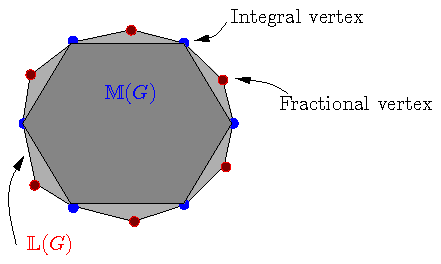
\includegraphics[width=0.8\textwidth]{fig/marginalpolytope.pdf}\cite{Wainwright2007}
\end{center}
\end{frame}

\begin{frame}
\vspace{1em}
\begin{center}
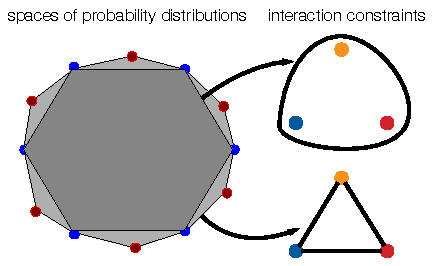
\includegraphics[width=0.7\textwidth]{fig/spacesandconstraints.pdf}\\
\end{center}
\end{frame}

	

	\section[PD comp]{Comparing modular and non-modular genotype-phenotype maps}
	% comparing spaces of probability distributions
% relating graphical models
% folder name: PDcomp

\begin{frame}
What is the relationship between the spaces of probability distributions defined on non-modular vs modular genotype-phenotype mappings?
\begin{center}
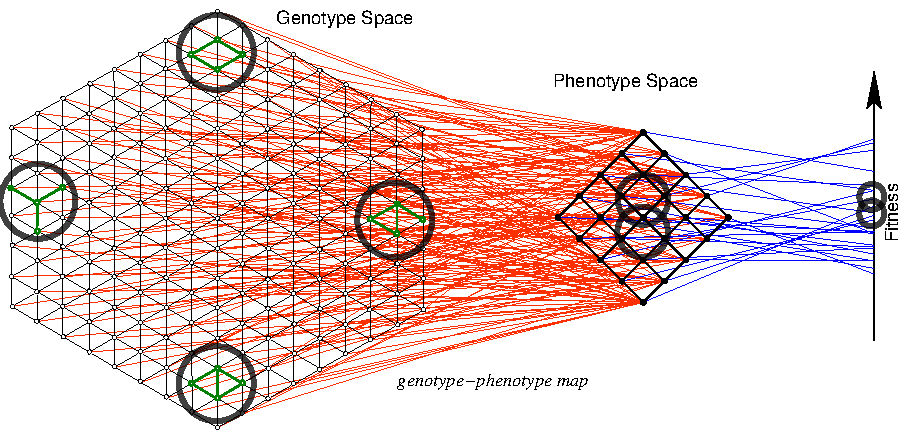
\includegraphics[width=0.8\textwidth]{fig/gpmapgraphs.pdf}
\end{center}
\end{frame}

\begin{frame}
\vspace{1em}
\begin{center}
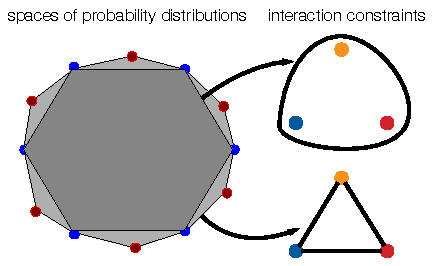
\includegraphics[width=0.7\textwidth]{fig/spacesandconstraints.pdf}\\
\end{center}
\end{frame}

\begin{frame}
\begin{center}
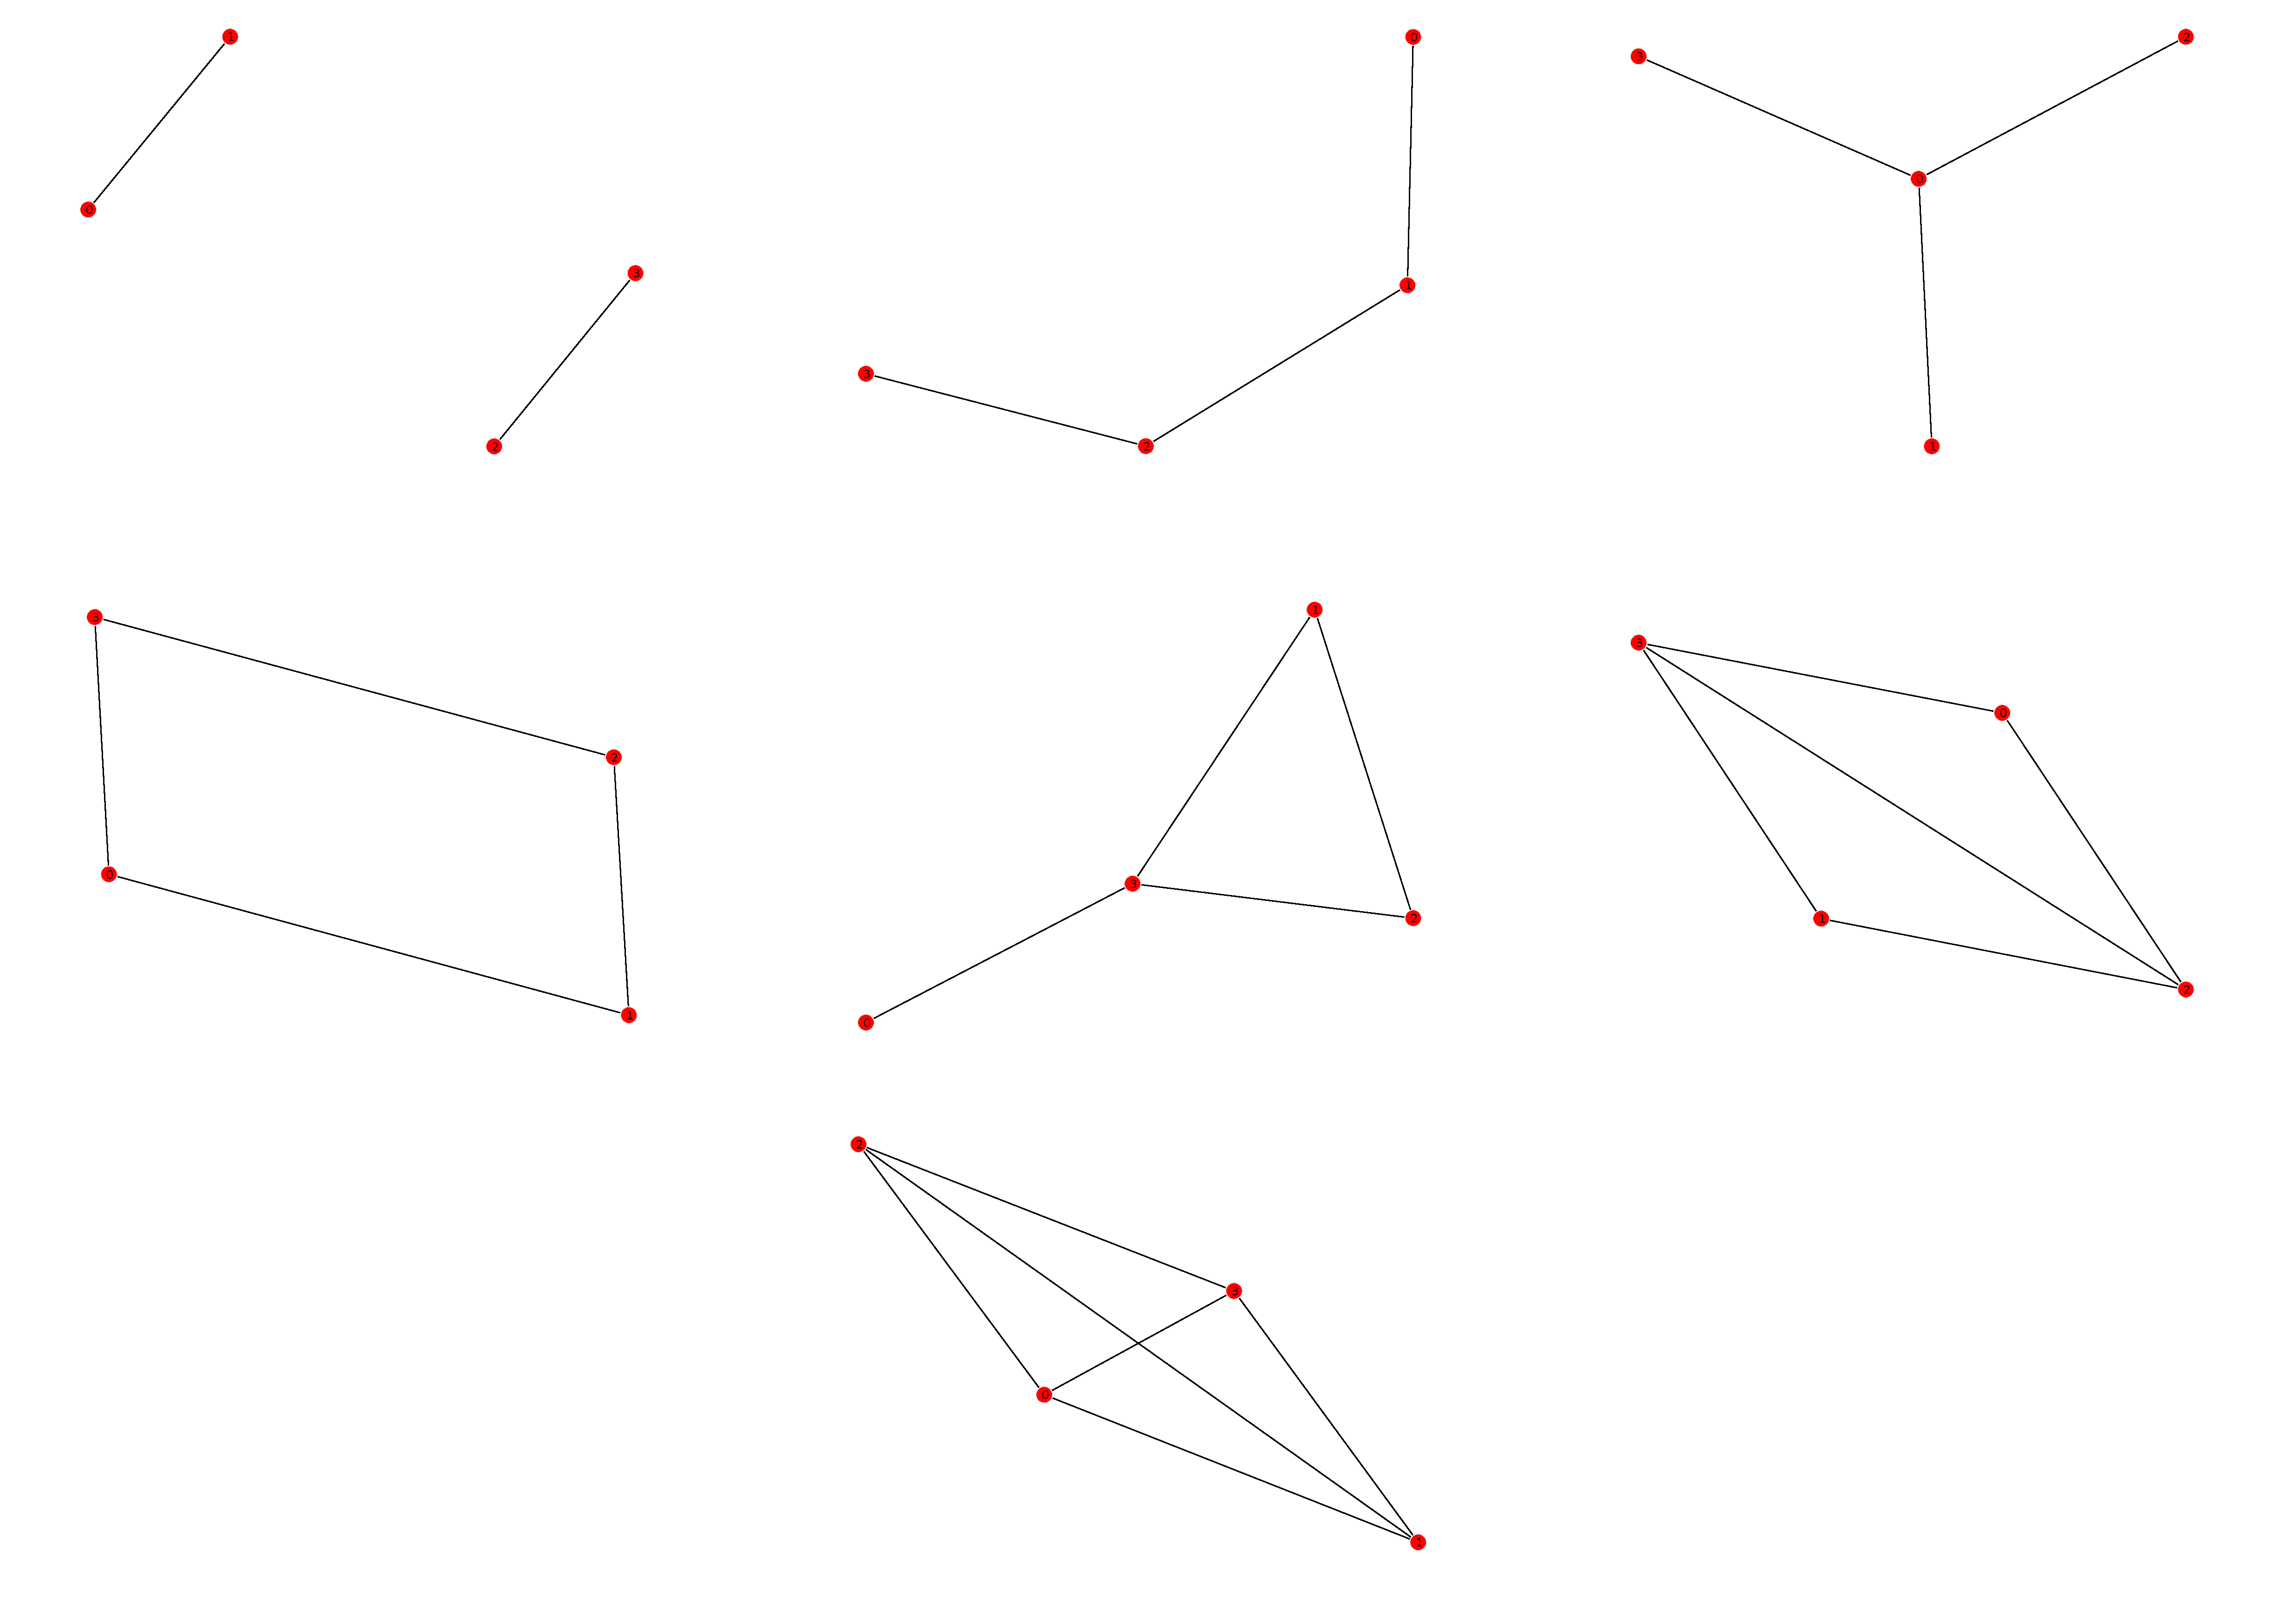
\includegraphics[width=0.9\textwidth]{fig/fourgraphs.pdf}
\end{center}
\end{frame}

\begin{frame}
\vspace{3em}
\begin{center}
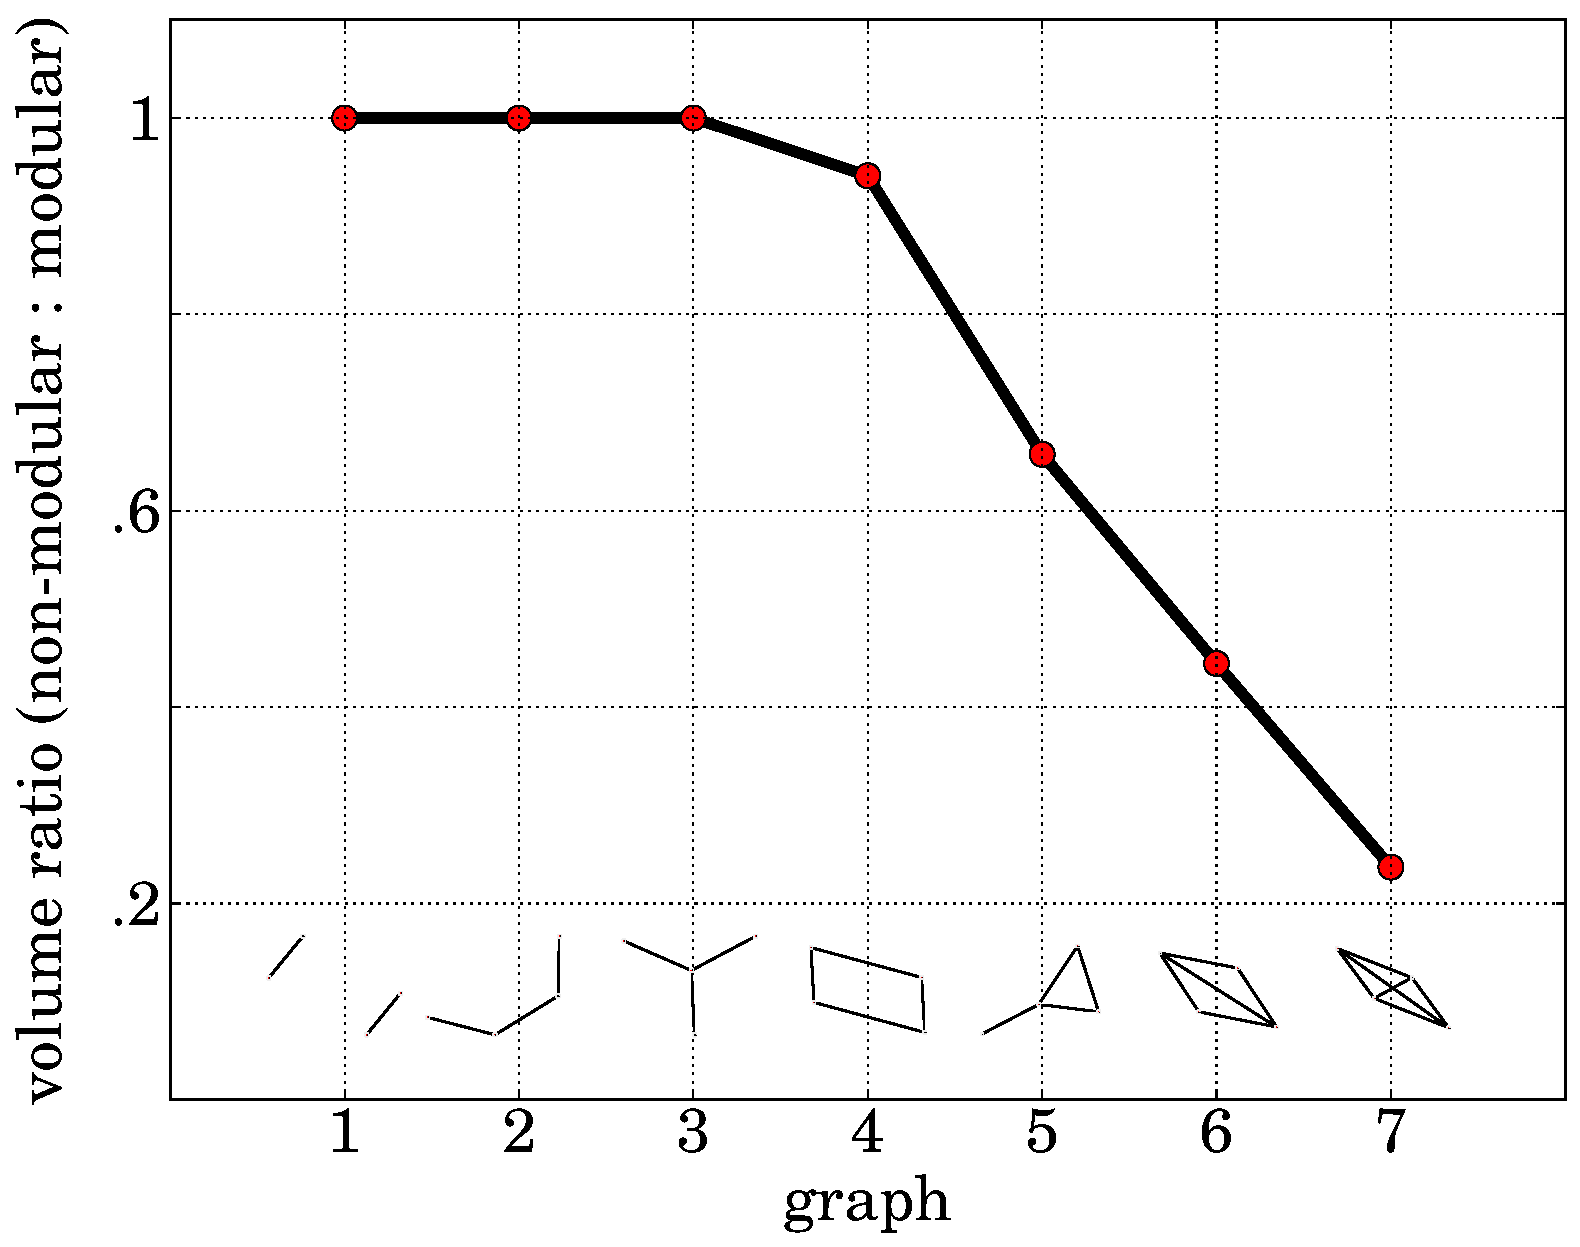
\includegraphics[width=0.8\textwidth]{fig/fourgraphsandplot.pdf}
\end{center}
\end{frame}

\begin{frame}
\begin{center}
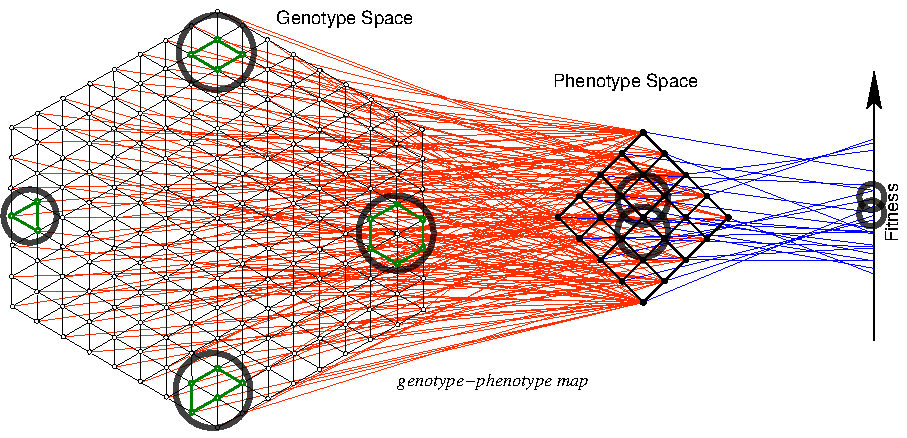
\includegraphics[width=0.9\textwidth]{fig/gpmapncycgraphs.pdf}
\end{center}
\end{frame}

\begin{frame}
\vspace{3em}
\begin{center}
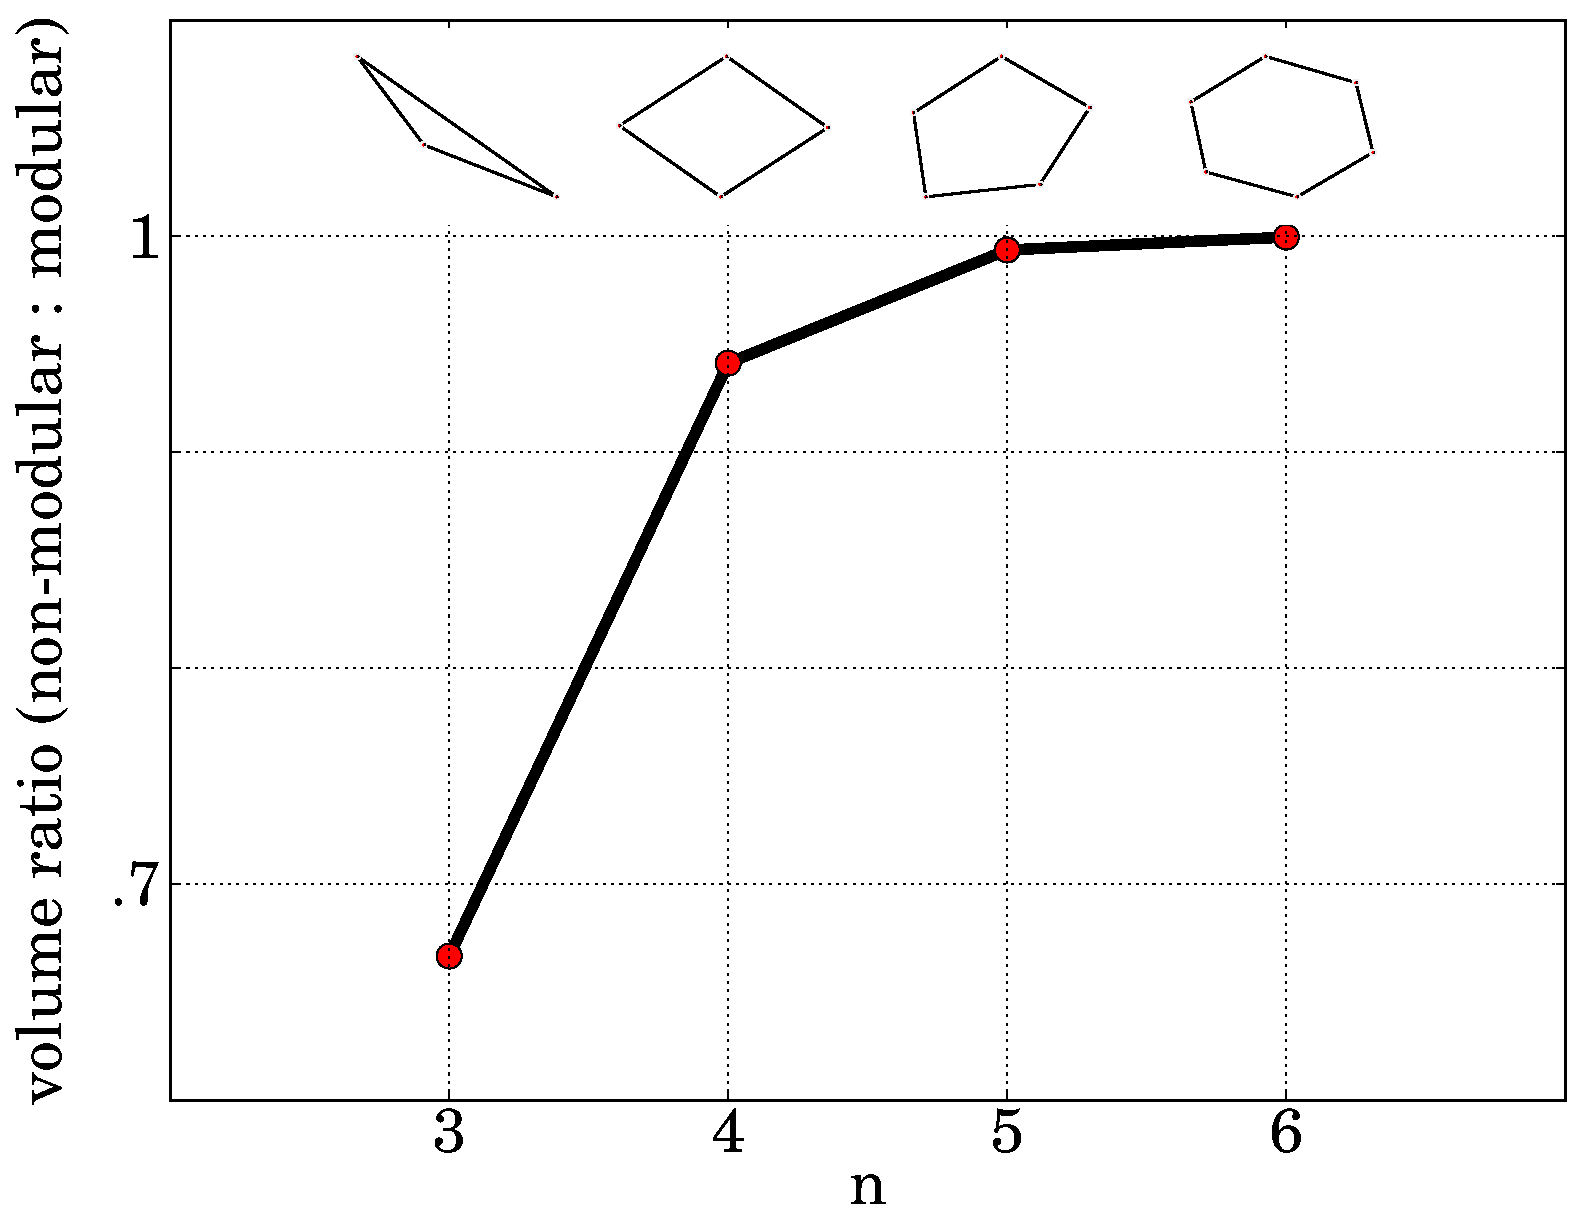
\includegraphics[width=0.8\textwidth]{fig/ncycgraphsandplot.pdf}
\end{center}
\end{frame}



	
	\begin{frame}
	\begin{block}{Conclusions}
	\begin{small}	
	\begin{itemize}
	\item For any tree-like (i.e. no cycles in the graphical representation) set of modules, the non-modular (global) and modular (local) spaces of probability distributions on genotype-phenotype mappings have equivalent volume and overlap completely
	\item For any collection of modules containing one or more cycles, the space of probability distributions on genotype-phenotype mappings accessed by the modular architecture relative to the non-modular architecture is \emph{larger}.
	\item For the n-cycle, as n increases, one approaches a linear chain and the difference between the modular and non-modular spaces of probability distributions shrinks to zero
	\item For those cases possessing nested cycles, the difference between the modular and non-modular spaces of probability distributions increases
	\end{itemize}		
	\end{small}
	\end{block}
	\end{frame}

	\begin{frame}
	\begin{footnotesize}	
	\begin{block}{Future work}
	\begin{itemize}
	\item compute non-modular:modular ratio for 
	\begin{enumerate}
	\begin{footnotesize}	
	\item more interesting network topologies on binary graphs
	\item graphs with higher-order edges (i.e. hypergraphs)
	\end{footnotesize}	
	\end{enumerate}	 
	\item examine topologies induced on spaces of genotypes, phenotypes and fitnesses by genotype-phenotype and phenotype-fitness mappings
	\item design an experiment at the conceptual level to clarify how these ideas can be tested in principle
	\item examine relationship to the general \textbf{marginal problem} connecting fields: logic, probability theory, algebraic geometry, machine learning, physics, and perhaps now also biology
	\item connect to the algebraic geometric approach to graphical models developed by Bernd Sturmfels (mathematics, UC Berkeley) and Reinhard Laubenbacher (biology, Virgina Tech): \emph{algebraic statistics}
	\end{itemize}		
	\end{block}
	\end{footnotesize}
	\end{frame}
	
	\begin{frame}
	\textbf{Acknowledgements}
	\begin{block}{Systems and Computational Biology}
	\begin{small}	
	\begin{itemize}
	\item Dan Biro
	\item Aviv Bergman
	\item Ximo Pechuan
	\end{itemize}		
	\end{small}
	\end{block}
	\begin{block}{Mathematics}
	\begin{small}	
	\begin{itemize}
	\item Jay Sulzberger :: logic and combinatorics
	\item Noson Yanofsky :: category theory
	\item Chirag Lakhani :: algebraic geometry
	\end{itemize}		
	\end{small}
	\end{block}
	\end{frame}
	
%	\section{References}
%	\begin{frame}
%\begin{block}{make friends with an expert in category theory}
%Have an expert review my manuscript on {\it Coherence constraints} that I have discussed today.
%\end{block}
%\begin{block}{implement graph transformations}
%Work toward a computational implementation of a model of the evolution of network representations of biological systems using algebraic graph transformations while maintaining a clear semantic interpretation of the representations used in terms of the BioPAX ontology.
%\end{block}
%\begin{block}{finish manuscript on functional closure and metabolic networks}
%Continue work on a second manuscript that builds upon the work of Robert Rosen to clarify the concept of functional (metabolic) closure and so-called intrinsic operationalism in metabolic networks.
%\end{block}
%\end{frame}

\begin{frame}[allowframebreaks]
        \frametitle{References}
        %\bibliographystyle{amsalpha}
        \bibliographystyle{unsrt} 
        %\bibliographystyle{numeric}
		\bibliography{bib/books,bib/papers}
\end{frame}
	
\end{document}